\documentclass[dvipdfmx]{jsarticle}
\setcounter{section}{1}
\setcounter{subsection}{0}
\usepackage{amsmath,amsfonts,amssymb,array,comment,mathtools,url,docmute}
\usepackage{longtable,booktabs,dcolumn,tabularx,mathtools,multirow,colortbl,xcolor}
\usepackage[dvipdfmx]{graphics}
\usepackage{bmpsize}
\usepackage{amsthm}
\usepackage{enumitem}
\setlistdepth{20}
\renewlist{itemize}{itemize}{20}
\setlist[itemize]{label=•}
\renewlist{enumerate}{enumerate}{20}
\setlist[enumerate]{label=\arabic*.}
\setcounter{MaxMatrixCols}{20}
\setcounter{tocdepth}{3}
\newcommand{\rotin}{\text{\rotatebox[origin=c]{90}{$\in $}}}
\newcommand{\amap}[6]{\text{\raisebox{-0.7cm}{\begin{tikzpicture} 
  \node (a) at (0, 1) {$\textstyle{#2}$};
  \node (b) at (#6, 1) {$\textstyle{#3}$};
  \node (c) at (0, 0) {$\textstyle{#4}$};
  \node (d) at (#6, 0) {$\textstyle{#5}$};
  \node (x) at (0, 0.5) {$\rotin $};
  \node (x) at (#6, 0.5) {$\rotin $};
  \draw[->] (a) to node[xshift=0pt, yshift=7pt] {$\textstyle{\scriptstyle{#1}}$} (b);
  \draw[|->] (c) to node[xshift=0pt, yshift=7pt] {$\textstyle{\scriptstyle{#1}}$} (d);
\end{tikzpicture}}}}
\newcommand{\twomaps}[9]{\text{\raisebox{-0.7cm}{\begin{tikzpicture} 
  \node (a) at (0, 1) {$\textstyle{#3}$};
  \node (b) at (#9, 1) {$\textstyle{#4}$};
  \node (c) at (#9+#9, 1) {$\textstyle{#5}$};
  \node (d) at (0, 0) {$\textstyle{#6}$};
  \node (e) at (#9, 0) {$\textstyle{#7}$};
  \node (f) at (#9+#9, 0) {$\textstyle{#8}$};
  \node (x) at (0, 0.5) {$\rotin $};
  \node (x) at (#9, 0.5) {$\rotin $};
  \node (x) at (#9+#9, 0.5) {$\rotin $};
  \draw[->] (a) to node[xshift=0pt, yshift=7pt] {$\textstyle{\scriptstyle{#1}}$} (b);
  \draw[|->] (d) to node[xshift=0pt, yshift=7pt] {$\textstyle{\scriptstyle{#2}}$} (e);
  \draw[->] (b) to node[xshift=0pt, yshift=7pt] {$\textstyle{\scriptstyle{#1}}$} (c);
  \draw[|->] (e) to node[xshift=0pt, yshift=7pt] {$\textstyle{\scriptstyle{#2}}$} (f);
\end{tikzpicture}}}}
\renewcommand{\thesection}{第\arabic{section}部}
\renewcommand{\thesubsection}{\arabic{section}.\arabic{subsection}}
\renewcommand{\thesubsubsection}{\arabic{section}.\arabic{subsection}.\arabic{subsubsection}}
\everymath{\displaystyle}
\allowdisplaybreaks[4]
\usepackage{vtable}
\theoremstyle{definition}
\newtheorem{thm}{定理}[subsection]
\newtheorem*{thm*}{定理}
\newtheorem{dfn}{定義}[subsection]
\newtheorem*{dfn*}{定義}
\newtheorem{axs}[dfn]{公理}
\newtheorem*{axs*}{公理}
\renewcommand{\headfont}{\bfseries}
\makeatletter
  \renewcommand{\section}{%
    \@startsection{section}{1}{\z@}%
    {\Cvs}{\Cvs}%
    {\normalfont\huge\headfont\raggedright}}
\makeatother
\makeatletter
  \renewcommand{\subsection}{%
    \@startsection{subsection}{2}{\z@}%
    {0.5\Cvs}{0.5\Cvs}%
    {\normalfont\LARGE\headfont\raggedright}}
\makeatother
\makeatletter
  \renewcommand{\subsubsection}{%
    \@startsection{subsubsection}{3}{\z@}%
    {0.4\Cvs}{0.4\Cvs}%
    {\normalfont\Large\headfont\raggedright}}
\makeatother
\makeatletter
\renewenvironment{proof}[1][\proofname]{\par
  \pushQED{\qed}%
  \normalfont \topsep6\p@\@plus6\p@\relax
  \trivlist
  \item\relax
  {
  #1\@addpunct{.}}\hspace\labelsep\ignorespaces
}{%
  \popQED\endtrivlist\@endpefalse
}
\makeatother
\renewcommand{\proofname}{\textbf{証明}}
\usepackage{tikz,graphics}
\usepackage[dvipdfmx]{hyperref}
\usepackage{pxjahyper}
\hypersetup{
 setpagesize=false,
 bookmarks=true,
 bookmarksdepth=tocdepth,
 bookmarksnumbered=true,
 colorlinks=false,
 pdftitle={},
 pdfsubject={},
 pdfauthor={},
 pdfkeywords={}}
\begin{document}
%\hypertarget{ux4f4dux76f8ux7a7aux9593}{%
\subsection{位相空間}%\label{ux4f4dux76f8ux7a7aux9593}}\par
%\hypertarget{ux4f4dux76f8}{%
\subsubsection{位相}%\label{ux4f4dux76f8}}
\begin{dfn}
1つの空集合でない集合$S$の部分集合系を$\mathfrak{O}$とおく。この集合$\mathfrak{O}$が次の3つの条件たちを満たすとき、その集合$\mathfrak{O}$はその集合$S$に1つの位相構造を定める、その集合$S$における1つの位相である、その集合$S$とその位相$\mathfrak{O}$との組$\left( S,\mathfrak{O} \right)$を位相空間、その集合$S$をその位相空間$\left( S,\mathfrak{O} \right)$の台集合、台など、その台集合$S$の元をその位相空間$\left( S,\mathfrak{O} \right)$の点、その集合$S$の部分集合をその位相空間$\left( S,\mathfrak{O} \right)$の部分集合という。
\begin{itemize}
\item
  $S,\emptyset \in \mathfrak{O}$が成り立つ。
\item
  $\forall O,P \in \mathfrak{O}$に対し、$O \cap P\in \mathfrak{O}$が成り立つ。
\item
  任意の添数集合$\varLambda$によって添数づけられたその集合$\mathfrak{O}$の元の族$\left\{ O_{\lambda} \right\}_{\lambda \in \varLambda}$において$\bigcup_{\lambda \in \varLambda} O_{\lambda}\in \mathfrak{O}$が成り立つ。
\end{itemize}
\end{dfn}\par
もちろん、次のように定義してもよい。
\begin{itemize}
\item
  $\forall O,P \in \mathfrak{O}$に対し、$O \cap P\in \mathfrak{O}$が成り立つ。
\item
  有限集合である添数集合$\varLambda$によって添数づけられたその集合$\mathfrak{O}$の元の族$\left\{ O_{\lambda} \right\}_{\scriptsize \begin{matrix}
  \lambda \in \varLambda \\
  {\#}\varLambda < \aleph_{0} \\
  \end{matrix}}$において$\bigcap_{\scriptsize \begin{matrix}
  \lambda \in \varLambda \\
  {\#}\varLambda < \aleph_{0} \\
  \end{matrix}} O_{\lambda}\in \mathfrak{O}$が成り立つ。
\end{itemize}\par
例えば、集合$\left\{ a,b,c \right\}$における位相は29つある\footnote{
\begin{align*}
&\left\{ \left\{ a,b,c \right\},\emptyset \right\},\\
&\left\{ \left\{ a,b,c \right\},\left\{ a \right\},\emptyset \right\},\left\{ \left\{ a,b,c \right\},\left\{ b \right\},\emptyset \right\},\left\{ \left\{ a,b,c \right\},\left\{ c \right\},\emptyset \right\},\\
&\left\{ \left\{ a,b,c \right\},\left\{ a,b \right\},\left\{ a \right\},\emptyset \right\},\left\{ \left\{ a,b,c \right\},\left\{ a,b \right\},\left\{ b \right\},\emptyset \right\},\\
&\left\{ \left\{ a,b,c \right\},\left\{ b,c \right\},\left\{ b \right\},\emptyset \right\},\left\{ \left\{ a,b,c \right\},\left\{ b,c \right\},\left\{ c \right\},\emptyset \right\},\\
&\left\{ \left\{ a,b,c \right\},\left\{ c,a \right\},\left\{ c \right\},\emptyset \right\},\left\{ \left\{ a,b,c \right\},\left\{ c,a \right\},\left\{ a \right\},\emptyset \right\},\\
&\left\{ \left\{ a,b,c \right\},\left\{ a,b \right\},\left\{ a \right\},\left\{ b \right\},\emptyset \right\},\left\{ \left\{ a,b,c \right\},\left\{ b,c \right\},\left\{ b \right\},\left\{ c \right\},\emptyset \right\},\ \left\{ \left\{ a,b,c \right\},\left\{ c,a \right\},\left\{ c \right\},\left\{ a \right\},\emptyset \right\},\\
&\left\{ \left\{ a,b,c \right\},\left\{ a,b \right\},\left\{ c \right\},\emptyset \right\},\left\{ \left\{ a,b,c \right\},\left\{ b,c \right\},\left\{ a \right\},\emptyset \right\},\ \left\{ \left\{ a,b,c \right\},\left\{ c,a \right\},\left\{ b \right\},\emptyset \right\},\\
&\left\{ \left\{ a,b,c \right\},\left\{ a,b \right\},\left\{ b,c \right\},\left\{ b \right\},\emptyset \right\},\left\{ \left\{ a,b,c \right\},\left\{ b,c \right\},\left\{ c,a \right\},\left\{ c \right\},\emptyset \right\},\ \left\{ \left\{ a,b,c \right\},\left\{ c,a \right\},\left\{ a,b \right\},\left\{ a \right\},\emptyset \right\},\\
&\left\{ \left\{ a,b,c \right\},\left\{ a,b \right\},\left\{ b,c \right\},\left\{ a \right\},\ \left\{ b \right\},\emptyset \right\},\left\{ \left\{ a,b,c \right\},\left\{ a,b \right\},\left\{ b,c \right\},\left\{ b \right\},\left\{ c \right\},\emptyset \right\},\\
&\left\{ \left\{ a,b,c \right\},\left\{ b,c \right\},\left\{ c,a \right\},\left\{ b \right\},\left\{ c \right\},\emptyset \right\},\left\{ \left\{ a,b,c \right\},\left\{ b,c \right\},\left\{ c,a \right\},\left\{ c \right\},\left\{ a \right\},\emptyset \right\},\\
&\left\{ \left\{ a,b,c \right\},\left\{ c,a \right\},\left\{ a,b \right\},\left\{ c \right\},\left\{ a \right\},\emptyset \right\},\ \left\{ \left\{ a,b,c \right\},\left\{ c,a \right\},\left\{ a,b \right\},\left\{ a \right\},\left\{ b \right\},\emptyset \right\},\\
&\left\{ \left\{ a,b,c \right\},\left\{ a,b \right\},\left\{ b,c \right\},\left\{ a \right\},\ \left\{ b \right\},\left\{ c \right\},\emptyset \right\},\\
&\left\{ \left\{ a,b,c \right\},\left\{ b,c \right\},\left\{ c,a \right\},\left\{ a \right\},\ \left\{ b \right\},\left\{ c \right\},\emptyset \right\},\\ 
&\left\{ \left\{ a,b,c \right\},\left\{ c,a \right\},\left\{ a,b \right\},\left\{ a \right\},\ \left\{ b \right\},\left\{ c \right\},\emptyset \right\},\\
&\left\{ \left\{ a,b,c \right\},\left\{ a,b \right\},\left\{ b,c \right\},\left\{ c,a \right\},\left\{ a \right\},\ \left\{ b \right\},\left\{ c \right\},\emptyset \right\} =\mathfrak{P}\left( \left\{ a,b,c \right\} \right)
\end{align*}
}。
\begin{thm}\label{8.1.1.1}
任意の集合$S$において、必ず$\mathfrak{O}_{*} = \left\{ \emptyset,S \right\}$、$\mathfrak{O}^{*}=\mathfrak{P}(S)$と2つの位相たちを考えることができその集合$S$における任意の位相$\mathfrak{O}$に対して次式が成り立つ。
\begin{align*}
\mathfrak{O}_{*}\subseteq \mathfrak{O \subseteq}\mathfrak{O}^{*}
\end{align*}
\end{thm}
\begin{proof} これは定義にあてはめれば、明らかであろう。
\end{proof}
\begin{dfn}
このような位相たち$\mathfrak{O}_{*}$、$\mathfrak{O}^{*}$をそれぞれその集合$S$における密着位相、離散位相といい、それらの位相空間たち$\left( S,\mathfrak{O}_{*} \right)$、$\left( S,\mathfrak{O}^{*} \right)$をそれぞれその集合$S$を台とする密着空間、離散空間という。
\end{dfn}
%\hypertarget{ux958bux96c6ux5408}{%
\subsubsection{開集合}%\label{ux958bux96c6ux5408}}
\begin{dfn}
1つの位相空間$\left( S,\mathfrak{O} \right)$においてその位相$\mathfrak{O}$に属する集合$O$をこの位相空間$\left( S,\mathfrak{O} \right)$の開集合という。位相空間$(S,\ \mathfrak{O})$の開集合全体の集合$\left\{ O \in \mathfrak{P}(S) \middle| O \in \mathfrak{O} \right\}$はまさしく位相$\mathfrak{O}$そのものでありこれをその位相空間$(S,\mathfrak{O})$の開集合系ともいう。
\end{dfn}
%\hypertarget{ux958bux6838}{%
\subsubsection{開核}%\label{ux958bux6838}}
\begin{dfn}
位相空間$\left( S,\mathfrak{O} \right)$が与えられたとき、$O \in \mathfrak{O}$かつ$O \subseteq M$なる集合$O$全体の和集合$\bigcup_{\scriptsize \begin{matrix}
O \in \mathfrak{O} \\
O \subseteq M \\
\end{matrix}} O$において、位相の定義より$\bigcup_{\scriptsize \begin{matrix}
O \in \mathfrak{O} \\
O \subseteq M \\
\end{matrix}} O\in \mathfrak{O}$が成り立つかつ、$\forall O \in \mathfrak{O}$に対し、$O \subseteq M$が成り立つなら、$O \subseteq \bigcup_{\scriptsize \begin{matrix}
O \in \mathfrak{O} \\
O \subseteq M \\
\end{matrix}} O$が成り立つ、即ち、その集合$\bigcup_{\scriptsize \begin{matrix}
O \in \mathfrak{O} \\
O \subseteq M \\
\end{matrix}} O$の大きさはいかなる、$O \subseteq M$が成り立つかつ、その位相$\mathfrak{O}$に属するような集合$O$の大きさ以上になる。これは後述する定理\ref{8.1.1.2}で改めて述べられるが、このような集合$\bigcup_{\scriptsize \begin{matrix}
O \in \mathfrak{O} \\
O \subseteq M \\
\end{matrix}} O$をその集合$M$の開核、内部、位相的内部といい${\mathrm{int}}M$、$\mathrm{Int}(M)$、$M^{\circ}$、$M^{i}$などと書く、即ち、次式のように定義される。この開核${\mathrm{int}}M$の元を内点という。もちろん、これはその集合$M$の元である。
\begin{align*}
S' = {\mathrm{int}}M \Leftrightarrow S' = \bigcup_{\scriptsize \begin{matrix}
O \in \mathfrak{O} \\
O \subseteq M \\
\end{matrix}} O\ \mathrm{if}\ M \in \mathfrak{P}(S)
\end{align*}
\end{dfn}\par
これは次の図のように考えると、分かりやすかろう。
\begin{center}
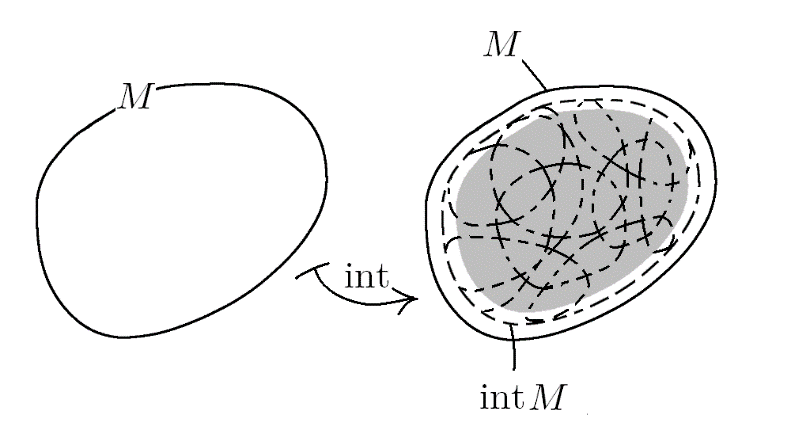
\includegraphics[width=93mm]{8.1.1.a.png}
\end{center}
\begin{thm}\label{8.1.1.2}
位相空間$\left( S,\mathfrak{O} \right)$において、$\forall M \in \mathfrak{P}(S)$に対し、その集合$M$の開核${\mathrm{int}}M$が集合$S'$であるならそのときに限り、次のこといずれも成り立つ、
\begin{itemize}
\item
  $S' \subseteq M$が成り立つ。
\item
  $S'\in \mathfrak{O}$が成り立つ。
\item
  $O \subseteq M$かつ$O \in \mathfrak{O}$が成り立つなら、$O \subseteq S'$が成り立つ。
\end{itemize}
さらに、順序集合$\left( \mathfrak{P}(S), \subseteq \right)$が与えられたとき、次式が成り立つ。
\begin{align*}
{\mathrm{int}}M = \max\left\{ O \in \mathfrak{O} \middle| O \subseteq M \right\}
\end{align*}
\end{thm}
\begin{proof}
位相空間$\left( S,\mathfrak{O} \right)$において、その集合$S$の任意の部分集合$M$の開核${\mathrm{int}}M$が集合$S'$であるなら、その集合$S'$はその集合$S$の部分集合で和集合$\bigcup_{\scriptsize \begin{matrix}
O \in \mathfrak{O} \\
O \subseteq M \\
\end{matrix}} O$に等しい。ここで、$O \subseteq M$が成り立つので、$\bigcup_{\scriptsize \begin{matrix}
O \in \mathfrak{O} \\
O \subseteq M \\
\end{matrix}} O \subseteq M$が成り立つかつ、$O \in \mathfrak{O}$と位相の定義より$\bigcup_{\scriptsize \begin{matrix}
O \in \mathfrak{O} \\
O \subseteq M \\
\end{matrix}} O\in \mathfrak{O}$が成り立つかつ、$O \subseteq M$なる任意のその位相$\mathfrak{O}$の元$O$に対し、$O \subseteq \bigcup_{\scriptsize \begin{matrix}
O \in \mathfrak{O} \\
O \subseteq M \\
\end{matrix}} O$が成り立つので、全称除去より$O \subseteq M \land O \in \mathfrak{O \Rightarrow}O \subseteq \bigcup_{\scriptsize \begin{matrix}
O \in \mathfrak{O} \\
O \subseteq M \\
\end{matrix}} O$が成り立つ。したがって、その集合$M$の開核${\mathrm{int}}M$が集合$S'$であるならそのときに限り、次のこといずれも成り立つ。
\begin{itemize}
\item
  $S' \subseteq M$が成り立つ。
\item
  $S'\in \mathfrak{O}$が成り立つ。
\item
  $O \subseteq M$かつ$O \in \mathfrak{O}$が成り立つなら、$O \subseteq S'$が成り立つ。
\end{itemize}\par
逆に、これらが成り立つなら、その和集合$\bigcup_{\scriptsize \begin{matrix}
O \in \mathfrak{O} \\
O \subseteq M \\
\end{matrix}} O$は上記の議論によりこれらを満たすので、その集合$S'$はその和集合$\bigcup_{\scriptsize \begin{matrix}
O \in \mathfrak{O} \\
O \subseteq M \\
\end{matrix}} O$とおくことができる。ここで、これらを満たすその和集合$\bigcup_{\scriptsize \begin{matrix}
O \in \mathfrak{O} \\
O \subseteq M \\
\end{matrix}} O$ではない集合$S''$が存在すると仮定すると、$S'' \subseteq M$かつ$S''\in \mathfrak{O}$が成り立つので、$S'' \subseteq \bigcup_{\scriptsize \begin{matrix}
O \in \mathfrak{O} \\
O \subseteq M \\
\end{matrix}} O$が成り立つが、これは$\bigcup_{\scriptsize \begin{matrix}
O \in \mathfrak{O} \\
O \subseteq M \\
\end{matrix}} O \subseteq M$かつ$\bigcup_{\scriptsize \begin{matrix}
O \in \mathfrak{O} \\
O \subseteq M \\
\end{matrix}} O\in \mathfrak{O}$が成り立つなら、$\bigcup_{\scriptsize \begin{matrix}
O \in \mathfrak{O} \\
O \subseteq M \\
\end{matrix}} O \subseteq S''$が成り立つことに矛盾する。したがって、その集合$S'$はその和集合$\bigcup_{\scriptsize \begin{matrix}
O \in \mathfrak{O} \\
O \subseteq M \\
\end{matrix}} O$である必要がありその集合$M$の開核${\mathrm{int}}M$が集合$S'$である。\par
さらに、順序集合$\left( \mathfrak{P}(S), \subseteq \right)$が与えられたとき、次のことが成り立つなら、
\begin{itemize}
\item
  ${\mathrm{int}}M \subseteq M$が成り立つ。
\item
  ${\mathrm{int}}M\in \mathfrak{O}$が成り立つ。
\item
  $O \subseteq M$かつ$O \in \mathfrak{O}$が成り立つなら、$O \subseteq {\mathrm{int}}M$が成り立つ。
\end{itemize}
これは次のように書き換えられることができる。
\begin{align*}
\forall O \in \left\{ O \in \mathfrak{O} \middle| O \subseteq M \right\}\left[ O \subseteq {\mathrm{int}}M \right]
\end{align*}
したがって、最大元の定義より次式が成り立つ。
\begin{align*}
{\mathrm{int}}M = \max\left\{ O \in \mathfrak{O} \middle| O \subseteq M \right\}
\end{align*}
\end{proof}
\begin{thm}\label{8.1.1.3}
位相空間$\left( S,\mathfrak{O} \right)$の開核について、次のことが成り立つ。
\begin{itemize}
\item
  $\forall M \in \mathfrak{P}(S)$に対し、$M \in \mathfrak{O}$が成り立つならそのときに限り、${\mathrm{int}}M = M$が成り立つ。
\item
  $\forall M,N \in \mathfrak{P}(S)$に対し、$M \subseteq N$が成り立つなら、${\mathrm{int}}M \subseteq {\mathrm{int}}N$が成り立つ。
\end{itemize}
\end{thm}
\begin{proof}
位相空間$\left( S,\mathfrak{O} \right)$が与えられたとき、$\forall M \in \mathfrak{P}(S)$に対し、$M \in \mathfrak{O}$が成り立つなら、$M \subseteq M$が成り立つかつ、$M \in \mathfrak{O}$が成り立つかつ、$O \subseteq M$かつ$O \in \mathfrak{O}$が成り立つなら、$O \subseteq M$が成り立つので、${\mathrm{int}}M = M$が成り立つ。逆に、${\mathrm{int}}M = M$が成り立つなら、$M \in \mathfrak{O}$が成り立つ。\par
$\forall M,N \in \mathfrak{P}(S)$に対し、$M \subseteq N$が成り立つときを考える。開核${\mathrm{int}}M$について、${\mathrm{int}}M \subseteq M$が成り立つかつ、${\mathrm{int}}M\in \mathfrak{O}$が成り立つかつ、$O \subseteq M$かつ$O \in \mathfrak{O}$が成り立つなら、$O \subseteq {\mathrm{int}}M$が成り立つ。開核${\mathrm{int}}N$についても同様である。以上より、${\mathrm{int}}M \subseteq M \subseteq N$が成り立つかつ、${\mathrm{int}}M\in \mathfrak{O}$が成り立つので、${\mathrm{int}}M \subseteq {\mathrm{int}}N$が成り立つ。
\end{proof}
%\hypertarget{ux9589ux96c6ux5408}{%
\subsubsection{閉集合}%\label{ux9589ux96c6ux5408}}
\begin{dfn}
位相空間$(S,\mathfrak{O})$において開集合のその集合$S$に対する補集合となるその集合$S$の部分集合をこの位相空間$\left( S,\mathfrak{O} \right)$の閉集合という。即ち、$S \setminus A \in \mathfrak{O}$なる集合$A$がその位相空間$\left( S,\mathfrak{O} \right)$の閉集合である。位相空間$(S,\ \mathfrak{O})$の閉集合全体の集合$\left\{ A \in \mathfrak{P}(S) \middle| S \setminus A \in \mathfrak{O} \right\}$をその位相空間$(S,\mathfrak{O})$の閉集合系という。
\end{dfn}
\begin{thm}\label{8.1.1.4}
位相空間$\left( S,\mathfrak{O} \right)$において、次のことが成り立つ。
\begin{itemize}
\item
  $S,\emptyset \in \mathfrak{A}$が成り立つ。
\item
  $\forall A,B \in \mathfrak{A}$に対し、$A \cup B \in \mathfrak{A}$が成り立つ。
\item
  任意の添数集合$\varLambda$によって添数づけられたその集合$\mathfrak{A}$の元の族$\left\{ A_{\lambda} \right\}_{\lambda \in \varLambda}$において$\bigcap_{\lambda \in \varLambda} A_{\lambda}\in \mathfrak{A}$が成り立つ。
\end{itemize}
\end{thm}
\begin{proof}
位相空間$(S,\mathfrak{O})$において、その位相空間$(S,\mathfrak{O})$の閉集合系を$\mathfrak{A}$と添数集合$\varLambda$によって添数づけられたそれらの集合$\mathfrak{O}$の元の族を$\left\{ O_{\lambda} \right\}_{\lambda \in \varLambda}$とし$A_{\lambda} = S \setminus O_{\lambda}$とおくと、添数集合$\varLambda$によって添数づけられたそれらの集合$\mathfrak{A}$の元の族$\left\{ A_{\lambda} \right\}_{\lambda \in \varLambda}$が得られる。したがって、次のようになる。
\begin{align*}
S,\emptyset \in \mathfrak{O \Leftrightarrow}S \setminus S,S \setminus \emptyset \in \mathfrak{O \Leftrightarrow}S,\emptyset \in \mathfrak{A}
\end{align*}
$\forall A,B \in \mathfrak{A}$に対し、次のようになる。
\begin{align*}
A,B \in \mathfrak{A} &\Leftrightarrow S \setminus A,S \setminus B \in \mathfrak{O}\\
&\Rightarrow S \setminus A \cap S \setminus B \in \mathfrak{O}\\
&\Leftrightarrow S \setminus (A \cup B)\in \mathfrak{O}\\
&\Leftrightarrow A \cup B \in \mathfrak{A}
\end{align*}
任意の添数集合$\varLambda$に対し、次のようになる。
\begin{align*}
\bigcup_{\lambda \in \varLambda} O_{\lambda}\in \mathfrak{O} &\Leftrightarrow S \setminus \bigcup_{\lambda \in \varLambda} O_{\lambda}\in \mathfrak{A}\\
&\Leftrightarrow \bigcap_{\lambda \in \varLambda} \left( S \setminus O_{\lambda} \right)\in \mathfrak{A}\\
&\Leftrightarrow \bigcap_{\lambda \in \varLambda} A_{\lambda}\in \mathfrak{A}
\end{align*}
\end{proof}
\begin{thm}\label{8.1.1.5}
その集合$S$の部分集合系$\mathfrak{A}$で上の3つの条件たちが満たされれば、その集合$\mathfrak{A}$が位相空間$\left( S,\mathfrak{O} \right)$の閉集合系と一致できるその位相$\mathfrak{O}$がただ1つに決まる。しかも、その位相$\mathfrak{O}$は次式を満たす。
\begin{align*}
\mathfrak{O}=\left\{ S \setminus A \in \mathfrak{P}(S) \middle| A \in \mathfrak{A} \right\}
\end{align*}
\end{thm}
\begin{proof}
その集合$S$の部分集合系$\mathfrak{A}$が次の3つの条件たちを満たすとしよう。
\begin{itemize}
\item
  $S,\emptyset \in \mathfrak{A}$が成り立つ。
\item
  $\forall A,B \in \mathfrak{A}$に対し、$A \cup B \in \mathfrak{A}$が成り立つ。
\item
  任意の添数集合$\varLambda$によって添数づけられたその集合$\mathfrak{A}$の元の族$\left\{ A_{\lambda} \right\}_{\lambda \in \varLambda}$において$\bigcap_{\lambda \in \varLambda} A_{\lambda}\in \mathfrak{A}$が成り立つ。
\end{itemize}
集合$\left\{ S \setminus A \in \mathfrak{P}(S) \middle| A \in \mathfrak{A} \right\}$を$\mathfrak{O}$とおくと、$S,\emptyset \in \mathfrak{A}$が成り立つなら、次のようになる。
\begin{align*}
S,\emptyset \in \mathfrak{A} &\Leftrightarrow S \setminus S,S \setminus \emptyset \in \mathfrak{O}\\
&\Leftrightarrow S,\emptyset \in \mathfrak{O}
\end{align*}
$\forall S \setminus A,S \setminus B \in \mathfrak{O}$に対し、$A \cup B \in \mathfrak{A}$が成り立つので、次のようになる。
\begin{align*}
S \setminus A \cap S \setminus B = S \setminus (A \cup B)\in \mathfrak{O}
\end{align*}
任意の添数集合$\varLambda$によって添数づけられたその集合$\mathfrak{O}$の元の族$\left\{ S \setminus A_{\lambda} \right\}_{\lambda \in \varLambda}$において、$\bigcap_{\lambda \in \varLambda} A_{\lambda}\in \mathfrak{A}$が成り立つので、次のようになる。
\begin{align*}
\bigcup_{\scriptsize \begin{matrix}
\lambda \in \varLambda \\
\end{matrix}} \left( S \setminus A_{\lambda} \right) = S \setminus \bigcap_{\lambda \in \varLambda} A_{\lambda}\in \mathfrak{O}
\end{align*}
以上より、その集合$\mathfrak{O}$は位相になる。\par
逆に、その位相$\mathfrak{O}$が与えられたとき、$\forall O \in \mathfrak{O}$に対し、次のようになる。
\begin{align*}
O \in \mathfrak{O} &\Leftrightarrow O \in \mathfrak{P}(S) \land S \setminus O \in \mathfrak{A}\\
&\Leftrightarrow S \setminus (S \setminus O)\in \mathfrak{P}(S) \land S \setminus O \in \mathfrak{A}
\end{align*}
したがって、その位相$\mathfrak{O}$がその集合$\mathfrak{A}$がその位相空間$\left( S,\mathfrak{O} \right)$の閉集合系と一致できる1つの位相$\mathfrak{O}$となっている。
\end{proof}
%\hypertarget{ux9589ux5305}{%
\subsubsection{閉包}%\label{ux9589ux5305}}
\begin{dfn}
位相空間$\left( S,\mathfrak{O} \right)$が与えられたとき、その位相空間$\left( S,\mathfrak{O} \right)$の閉集合系$\mathfrak{A}$を用いて$A \in \mathfrak{A}$かつ$M \subseteq A$なる集合$A$全体の積集合$\bigcap_{\scriptsize \begin{matrix}
A \in \mathfrak{A} \\
M \subseteq A \\
\end{matrix}} A$において、上記の閉集合についての定理より$\bigcap_{\scriptsize \begin{matrix}
A \in \mathfrak{A} \\
M \subseteq A \\
\end{matrix}} A\in \mathfrak{A}$が成り立つかつ、$\forall A \in \mathfrak{A}$に対し、$M \subseteq A$が成り立つなら、$\bigcap_{\scriptsize \begin{matrix}
A \in \mathfrak{A} \\
M \subseteq A \\
\end{matrix}} A \subseteq A$が成り立つ、即ち、その集合$\bigcap_{\scriptsize \begin{matrix}
A \in \mathfrak{A} \\
M \subseteq A \\
\end{matrix}} A$の大きさはいかなる、$M \subseteq A$が成り立つかつ、その閉集合系$\mathfrak{A}$に属するような集合$A$の大きさ以下になる。これは後述する定理\ref{8.1.1.6}で改めて述べられるが、このような集合$\bigcap_{\scriptsize \begin{matrix}
A \in \mathfrak{A} \\
M \subseteq A \\
\end{matrix}} A$をその集合$M$の閉包、触集合といい${\mathrm{cl}}M$、$Cl(M)$、$\overline{M}$、$M^{a}$などと書く、即ち、次式のように定義される。この閉包${\mathrm{cl}}M$の元を触点という。もちろん、その集合$M$の任意の元はその閉包${\mathrm{cl}}M$の触点である。
\begin{align*}
{\mathrm{cl}}M = \bigcap_{\scriptsize \begin{matrix}
A \in \mathfrak{A} \\
M \subseteq A \\
\end{matrix}} A
\end{align*}
\end{dfn}\par
これは次の図のように考えると、分かりやすかろう。
\begin{center}
  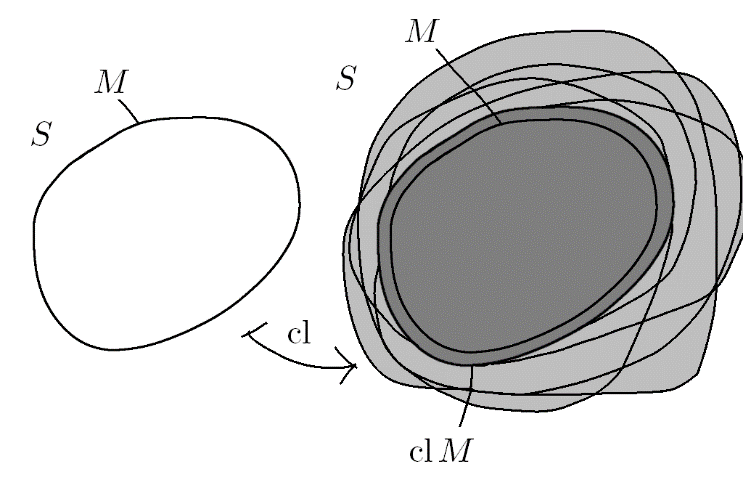
\includegraphics[width=86mm]{8.1.1.b.png}
\end{center}
\begin{thm}\label{8.1.1.6}
位相空間$\left( S,\mathfrak{O} \right)$において、$\forall M \in \mathfrak{P}(S)$に対し、その集合$M$の閉包${\mathrm{cl}}M$が集合$S'$であるならそのときに限り、次のこといずれも成り立つ。
\begin{itemize}
\item
  $M \subseteq S'$が成り立つ。
\item
  $S'\in \mathfrak{A}$が成り立つ。
\item
  $M \subseteq A$かつ$A \in \mathfrak{A}$が成り立つなら、$S' \subseteq A$が成り立つ。
\end{itemize}
さらに、順序集合$\left( \mathfrak{P}(S), \subseteq \right)$が与えられたとき、次式が成り立つ。
\begin{align*}
{\mathrm{cl}}M = \min\left\{ A \in \mathfrak{A} \middle| M \subseteq A \right\}
\end{align*}
\end{thm}
\begin{proof}
位相空間$\left( S,\mathfrak{O} \right)$において、その位相空間$\left( S,\mathfrak{O} \right)$の閉集合系$\mathfrak{A}$を用いてその集合$S$の任意の部分集合$M$の閉包${\mathrm{cl}}M$が集合$S'$であるなら、その集合$S'$はその集合$S$の部分集合で積集合$\bigcap_{\scriptsize \begin{matrix}
A \in \mathfrak{A} \\
M \subseteq A \\
\end{matrix}} A$に等しい。ここで、$M \subseteq A$が成り立つので、$M \subseteq \bigcap_{\scriptsize \begin{matrix}
A \in \mathfrak{A} \\
M \subseteq A \\
\end{matrix}} A$が成り立つかつ、$A \in \mathfrak{A}$と閉集合についての定理より$\bigcap_{\scriptsize \begin{matrix}
A \in \mathfrak{A} \\
M \subseteq A \\
\end{matrix}} A\in \mathfrak{A}$が成り立つかつ、$M \subseteq A$なる任意のその閉集合系$\mathfrak{A}$の元$A$に対し、$\bigcap_{\scriptsize \begin{matrix}
A \in \mathfrak{A} \\
M \subseteq A \\
\end{matrix}} A \subseteq A$が成り立つので、全称除去より$M \subseteq A \land A \in \mathfrak{A \Rightarrow}\bigcap_{\scriptsize \begin{matrix}
A \in \mathfrak{A} \\
M \subseteq A \\
\end{matrix}} A \subseteq A$が成り立つ。したがって、その集合$M$の閉包${\mathrm{cl}}M$が集合$S'$であるならそのときに限り、次のこといずれも成り立つ。
\begin{itemize}
\item
  $M \subseteq S'$が成り立つ。
\item
  $S'\in \mathfrak{A}$が成り立つ。
\item
  $M \subseteq A$かつ$A \in \mathfrak{A}$が成り立つなら、$S' \subseteq A$が成り立つ。
\end{itemize}\par
逆に、これらが成り立つなら、その積集合$\bigcap_{\scriptsize \begin{matrix}
A \in \mathfrak{A} \\
M \subseteq A \\
\end{matrix}} A$は上記の議論によりこれらを満たすので、その集合$S'$はその積集合$\bigcap_{\scriptsize \begin{matrix}
A \in \mathfrak{A} \\
M \subseteq A \\
\end{matrix}} A$とおくことができる。ここで、これらを満たすその積集合$\bigcap_{\scriptsize \begin{matrix}
A \in \mathfrak{A} \\
M \subseteq A \\
\end{matrix}} A$ではない集合$S''$が存在すると仮定すると、$M \subseteq S''$かつ$S''\in \mathfrak{A}$が成り立つので、$\bigcap_{\scriptsize \begin{matrix}
A \in \mathfrak{A} \\
M \subseteq A \\
\end{matrix}} A \subseteq S''$が成り立つが、これは$M \subseteq \bigcap_{\scriptsize \begin{matrix}
A \in \mathfrak{A} \\
M \subseteq A \\
\end{matrix}} A$かつ$\bigcap_{\scriptsize \begin{matrix}
A \in \mathfrak{A} \\
M \subseteq A \\
\end{matrix}} A\in \mathfrak{A}$が成り立つなら、$S'' \subseteq \bigcap_{\scriptsize \begin{matrix}
A \in \mathfrak{A} \\
M \subseteq A \\
\end{matrix}} A$が成り立つことに矛盾する。したがって、その集合$S'$はその積集合$\bigcap_{\scriptsize \begin{matrix}
A \in \mathfrak{A} \\
M \subseteq A \\
\end{matrix}} A$である必要がありその集合$M$の閉包${\mathrm{cl}}M$が集合$S'$である。\par
さらに、順序集合$\left( \mathfrak{P}(S), \subseteq \right)$が与えられたとき、次のことが成り立つなら、
\begin{itemize}
\item
  $M \subseteq {\mathrm{cl}}M$が成り立つ。
\item
  ${\mathrm{cl}}M\in \mathfrak{A}$が成り立つ。
\item
  $M \subseteq A$かつ$A \in \mathfrak{A}$が成り立つなら、${\mathrm{cl}}M \subseteq A$が成り立つ。
\end{itemize}
これは次のように書き換えられることができる。
\begin{align*}
\forall A \in \left\{ A \in \mathfrak{A} \middle| M \subseteq A \right\}\left[ {\mathrm{cl}}M \subseteq A \right]
\end{align*}
したがって、最小元の定義より次式が成り立つ。
\begin{align*}
{\mathrm{cl}}M = \min\left\{ A \in \mathfrak{A} \middle| M \subseteq A \right\}
\end{align*}
\end{proof}
\begin{thm}\label{8.1.1.7}
位相空間$\left( S,\mathfrak{O} \right)$の閉包について次のことが成り立つ。
\begin{itemize}
\item
  $\forall M \in \mathfrak{P}(S)$に対し、$M \in \mathfrak{A}$が成り立つならそのときに限り、${\mathrm{cl}}M = M$が成り立つ。
\item
  $\forall M,N \in \mathfrak{P}(S)$に対し、$M \subseteq N$が成り立つなら、${\mathrm{cl}}M \subseteq {\mathrm{cl}}N$が成り立つ。
\end{itemize}
\end{thm}
\begin{proof}
位相空間$\left( S,\mathfrak{O} \right)$が与えられたとき、その位相空間$\left( S,\mathfrak{O} \right)$の閉集合系$\mathfrak{A}$を用いて$\forall M \in \mathfrak{P}(S)$に対し、$M \in \mathfrak{A}$が成り立つなら、$M \subseteq M$が成り立つかつ、$M \in \mathfrak{A}$が成り立つかつ、$M \subseteq A$かつ$A \in \mathfrak{A}$が成り立つなら、$M \subseteq A$が成り立つので、${\mathrm{cl}}M = M$が成り立つ。逆に、${\mathrm{cl}}M = M$が成り立つなら、$M \in \mathfrak{A}$が成り立つ。\par
$\forall M,N \in \mathfrak{P}(S)$に対し、$M \subseteq N$が成り立つときを考える。閉包${\mathrm{cl}}M$について、${\mathrm{cl}}M \supseteq M$が成り立つかつ、${\mathrm{cl}}M\in \mathfrak{A}$が成り立つかつ、$M \subseteq A$かつ$A \in \mathfrak{A}$が成り立つなら、${\mathrm{cl}}M \subseteq A$が成り立つ。閉包${\mathrm{cl}}N$についても同様である。以上より、$M \subseteq N \subseteq {\mathrm{cl}}N$が成り立つかつ、${\mathrm{cl}}N\in \mathfrak{A}$が成り立つので、${\mathrm{cl}}M \subseteq {\mathrm{cl}}N$が成り立つ。
\end{proof}
%\hypertarget{ux958bux6838ux3068ux9589ux5305ux3068ux306eux95a2ux4fc2}{%
\subsubsection{開核と閉包との関係}%\label{ux958bux6838ux3068ux9589ux5305ux3068ux306eux95a2ux4fc2}}
\begin{thm}\label{8.1.1.8}
位相空間$\left( S,\mathfrak{O} \right)$と$M \in \mathfrak{P}(S)$なる集合$M$において、次式たちが成り立つ。このことをここでは開核と閉包との関係と呼ぶことにする\footnote{別の表記を用いれば、次のようになる。
\begin{align*}
  M^{ca} &= M^{ic}\\
  M^{cac} &= M^{i}\\
  M^{ci} &= M^{ac}\\
  M^{cic} &= M^{a}
\end{align*}}。
\begin{align*}
{\mathrm{cl}}(S \setminus M) &= S \setminus {\mathrm{int}}M\\
S \setminus {\mathrm{cl}}(S \setminus M) &= {\mathrm{int}}M\\
{\mathrm{int}}(S \setminus M) &= S \setminus {\mathrm{cl}}M\\
S \setminus {\mathrm{int}}(S \setminus M) &= {\mathrm{cl}}M
\end{align*}
\end{thm}\par
これは次の図のように考えると、分かりやすかろう。
\begin{center}
  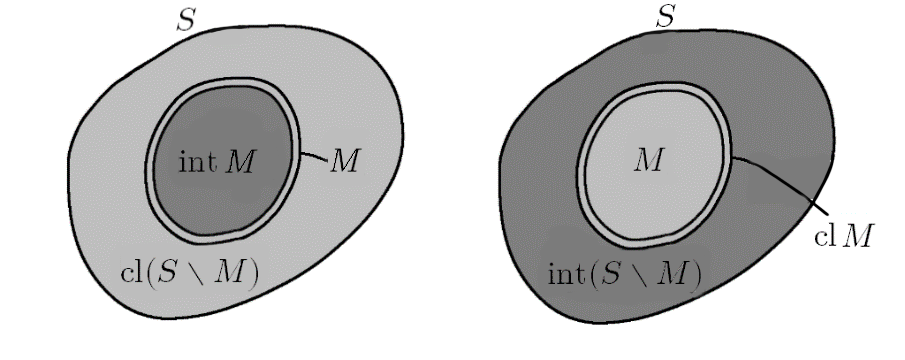
\includegraphics[width=104mm]{8.1.1.c.png}
\end{center}
ちなみに、1つの位相空間$\left( S,\mathfrak{O} \right)$において$S$対$\emptyset$、$\mathrm{int}$対$\mathrm{cl}$、$\cup$対$\cap$、$\subseteq$対$\supseteq$を交互に入れ替えたものも成り立つことが知られており、この性質を位相的双対律という。
\begin{proof}
位相空間$\left( S,\mathfrak{O} \right)$と$\forall M \in \mathfrak{P}(S)$なる集合$M$において、その位相空間$\left( S,\mathfrak{O} \right)$の閉集合系を$\mathfrak{A}$とおけば、$\forall A \in \mathfrak{A}$に対し${\mathrm{int}}M \subseteq M$より$S \setminus M \subseteq S \setminus {\mathrm{int}}M$が得られ、${\mathrm{int}}M = S \setminus S \setminus {\mathrm{int}}M\in \mathfrak{O}$と閉集合の定義より$S \setminus {\mathrm{int}}M\in \mathfrak{A}$が得られる。ここで、$S \setminus M \subseteq A$なる任意の閉集合$A$を考えると、$S \setminus A \subseteq S \setminus S \setminus M = M$と閉集合の定義より$S \setminus A \in \mathfrak{O}$かつ$S \setminus A \subseteq M$が得られる。ここで、その集合${\mathrm{int}}M$は$O \in \mathfrak{O}$かつ$O \subseteq M$なる開集合$O$全体の和集合$\bigcup_{\scriptsize \begin{matrix}
O \in \mathfrak{O} \\
O \subseteq M \\
\end{matrix}} O$でありその集合${\mathrm{int}}M$の大きさはいかなる、$O \subseteq M$が成り立つかつ、その位相$\mathfrak{O}$に属するような集合$O$の大きさ以上になるのであったので、$S \setminus A \subseteq {\mathrm{int}}M$が成り立つ。したがって、$S \setminus {\mathrm{int}}M\in \mathfrak{A}$かつ$S \setminus {\mathrm{int}}M \subseteq S \setminus S \setminus A = A$が得られる。ここで、その集合${\mathrm{cl}}(S \setminus M)$は$A \in \mathfrak{A}$かつ$S \setminus M \subseteq A$なる閉集合$A$全体の積集合$\bigcap_{\scriptsize \begin{matrix}
A \in \mathfrak{A} \\
M \subseteq A \\
\end{matrix}} A$でありその集合${\mathrm{cl}}(S \setminus M)$の大きさはいかなる、$M \subseteq A$が成り立つかつ、その閉集合系$\mathfrak{A}$に属するような集合$A$の大きさ以下になるのであったので、${\mathrm{cl}}(S \setminus M) = S \setminus {\mathrm{int}}M$が成り立つ。\par
これが用いられると、次のようになる。
\begin{align*}
S \setminus {\mathrm{cl}}(S \setminus M) &= S \setminus S \setminus {\mathrm{int}}M\\
&= {\mathrm{int}}M\\
{\mathrm{int}}(S \setminus M) &= S \setminus S \setminus {\mathrm{int}}(S \setminus M)\\
&= S \setminus {\mathrm{cl}}(S \setminus S \setminus M)\\
&= S \setminus {\mathrm{cl}}M\\
S \setminus {\mathrm{int}}(S \setminus M) &= {\mathrm{cl}}(S \setminus S \setminus M)\\
&= {\mathrm{cl}}M
\end{align*}
\end{proof}
\begin{thm}\label{8.1.1.9}
位相空間$\left( S,\mathfrak{O} \right)$が与えられたとする。$\forall a \in S$に対し、$a \in {\mathrm{cl}}M$が成り立つならそのときに限り、$\forall O \in \mathfrak{O}$に対し、$a \in O$が成り立つなら、$O \cap M \neq \emptyset$が成り立つ。
\end{thm}
\begin{proof}
位相空間$\left( S,\mathfrak{O} \right)$が与えられたとする。$\forall a \in S$に対し、$a \in {\mathrm{cl}}M$が成り立たないなら、$a \in S \setminus {\mathrm{cl}}M$が成り立つ。したがって、$a \in {\mathrm{int}}(S \setminus M)$が成り立つことになりその集合${\mathrm{int}}(S \setminus M)$はその位相$\mathfrak{O}$の開集合で${\mathrm{int}}(S \setminus M) \subseteq S \setminus M$が成り立つことから、次のようになるので、
\begin{align*}
{\mathrm{int}}(S \setminus M) \cap M \subseteq S \setminus M \cap M = \emptyset
\end{align*}
${\mathrm{int}}(S \setminus M) = \emptyset$が成り立つ。\par
逆に、$\exists O \in \mathfrak{O}$に対し、$O \cap M = \emptyset$が成り立つなら、$\forall a \in O$に対し、$a \in O$かつ$a \notin O \cap P$が成り立つことになり、したがって、$a \in O$かつ$a \notin M$が成り立つので、$O \subseteq S \setminus M$が成り立つ。ここで、その集合$O$が開集合で$O = {\mathrm{int}}O$が成り立つことに注意すれば、$O \subseteq {\mathrm{int}}(S \setminus M)$が成り立ち、${\mathrm{int}}(S \setminus M) = S \setminus {\mathrm{cl}}M$が成り立つので、その元$a$はその閉包${\mathrm{cl}}M$に属さない。\par
以上対偶律により、$\forall a \in S$に対し、$a \in {\mathrm{cl}}M$が成り立つならそのときに限り、$\forall O \in \mathfrak{O}$に対し、$a \in O$が成り立つなら、$O \cap M \neq \emptyset$が成り立つ。
\end{proof}
\begin{thm}\label{8.1.1.10}
位相空間$\left( S,\mathfrak{O} \right)$が与えられたとする。このとき、次のことが成り立つ。
\begin{itemize}
\item
  $\forall O \in \mathfrak{O\forall}M \in \mathfrak{P}(S)$に対し、$O \cap {\mathrm{cl}}M \subseteq {\mathrm{cl}}(O \cap M)$が成り立つ。
\item
  $\forall O \in \mathfrak{O\forall}M \in \mathfrak{P}(S)$に対し、$O \cap M = \emptyset$が成り立つなら、$O \cap {\mathrm{cl}}M = \emptyset$が成り立つ。
\end{itemize}
\end{thm}
\begin{proof} 位相空間$\left( S,\mathfrak{O} \right)$が与えられたとする。\par
$\forall O \in \mathfrak{O\forall}M \in \mathfrak{P}(S)\forall a \in O \cap {\mathrm{cl}}M$に対し、明らかに$a \in {\mathrm{cl}}M$が成り立ち、$a \in O'$なるその位相$\mathfrak{O}$の任意の開集合$O'$が与えられると、位相の定義よりその集合$O \cap O'$も開集合で$O \cap O' \cap M \neq \emptyset$が成り立つ。したがって、$a \in O'$なるその位相$\mathfrak{O}$の任意の開集合たち$O'$に対し、$O' \cap (O \cap M) \neq \emptyset$が成り立つので、$a \in {\mathrm{cl}}(O \cap M)$が成り立つ。以上より、$O \cap {\mathrm{cl}}M \subseteq {\mathrm{cl}}(O \cap M)$が成り立つ。\par
特に、$O \cap M = \emptyset$が成り立つなら、上記の議論により$O \cap {\mathrm{cl}}M \subseteq {\mathrm{cl}}\emptyset$が成り立つかつ、空集合$\emptyset$はその位相空間$\left( S,\mathfrak{O} \right)$での閉集合でもあるので、${\mathrm{cl}}\emptyset = \emptyset$が成り立つことになり、したがって、$O \cap {\mathrm{cl}}M = \emptyset$が成り立つ。
\end{proof}
%\hypertarget{ux958bux6838ux4f5cux7528ux5b50ux3068ux9589ux5305ux4f5cux7528ux5b50}{%
\subsubsection{開核作用子と閉包作用子}%\label{ux958bux6838ux4f5cux7528ux5b50ux3068ux9589ux5305ux4f5cux7528ux5b50}}
\begin{dfn}
位相空間$\left( S,\mathfrak{O} \right)$において、写像$int\mathfrak{:P}(S)\mathfrak{\rightarrow P}(S);M \mapsto int(M)$をその位相空間$\left( S,\mathfrak{O} \right)$における開核作用子という。
\end{dfn}
\begin{thm}\label{8.1.1.11}
位相空間$\left( S,\mathfrak{O} \right)$が与えられたとき、次のことが成り立つ。
\begin{itemize}
\item
  ${\mathrm{int}}S = S$が成り立つ。
\item
  $\forall M\in \mathfrak{P}(S)$に対し、${\mathrm{int}}M \subseteq M$が成り立つ。
\item
  $\forall M,N\in \mathfrak{P}(S)$に対し、${\mathrm{int}}(M \cap N) = {\mathrm{int}}M \cap {\mathrm{int}}N$が成り立つ。
\item
  $\forall M\in \mathfrak{P}(S)$に対し、${\mathrm{int}}{{\mathrm{int}}M} = {\mathrm{int}}M$が成り立つ。
\end{itemize}
\end{thm}\par
これは次の図のように考えると、分かりやすかろう。
\begin{center}
  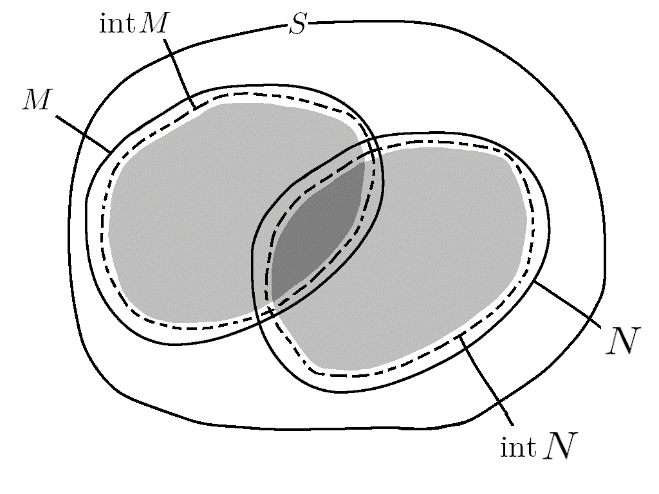
\includegraphics[width=80mm]{8.1.1.d.png}
\end{center}
\begin{proof} 位相空間$\left( S,\mathfrak{O} \right)$において、定理\ref{8.1.1.2}より$S \subseteq S$かつ$S \in \mathfrak{O}$かつ$O \subseteq S \land O \in \mathfrak{O} \Rightarrow O \subseteq S$が成り立つので、${\mathrm{int}}S = S$が得られる。\par
$\forall M \in \mathfrak{P}(S)$に対し、定義より明らかに${\mathrm{int}}M \subseteq M$が成り立つ。\par
これにより、$\forall M,N \in \mathfrak{P}(S)$に対し、${\mathrm{int}}M \cap {\mathrm{int}}N \subseteq M \cap N$が成り立つ。ここで、位相の定義と${\mathrm{int}}M,{\mathrm{int}}N\in \mathfrak{O}$より${\mathrm{int}}M \cap {\mathrm{int}}N\in \mathfrak{O}$が成り立つかつ、$O \subseteq M \cap N$なる任意の開集合$O$を考えると、$O \subseteq M$かつ$O \in \mathfrak{O}$が成り立つなら、$O \subseteq {\mathrm{int}}M$が成り立つことと$O \subseteq N$かつ$O \in \mathfrak{O}$が成り立つなら、$O \subseteq {\mathrm{int}}N$が成り立つことより$O \subseteq {\mathrm{int}}M \cap {\mathrm{int}}N$が得られる。したがって、定理\ref{8.1.1.2}より${\mathrm{int}}(M \cap N) = {\mathrm{int}}M \cap {\mathrm{int}}N$が成り立つ。\par
$\forall M\in \mathfrak{P}(S)$に対し、${\mathrm{int}}M \subseteq {\mathrm{int}}M$かつ${\mathrm{int}}M\in \mathfrak{O}$が成り立つかつ、$O \subseteq {\mathrm{int}}M$かつ$O \in \mathfrak{O}$が成り立つなら、$O \subseteq {\mathrm{int}}M$が成り立つことより${\mathrm{int}}{{\mathrm{int}}M} = {\mathrm{int}}M$が得られる。
\end{proof}
\begin{thm}\label{8.1.1.12}
空集合$\emptyset$でない集合$S$の各部分集合たちにその集合$S$の部分集合たちを対応させる写像$i:\mathfrak{P}(S)\mathfrak{\rightarrow P}(S)$で次のことが成り立つとする。
\begin{itemize}
\item
  $i(S) = S$が成り立つ。
\item
  $\forall M\in \mathfrak{P}(S)$に対し、$i(M) \subseteq M$が成り立つ。
\item
  $\forall M,N\in \mathfrak{P}(S)$に対し、$i(M \cap N) = i(M) \cap i(N)$が成り立つ。
\item
  $i \circ i = i$が成り立つ。
\end{itemize}
このとき、その写像$i$がその位相空間$\left( S,\mathfrak{O} \right)$における開核作用子と一致できる1つの位相$\mathfrak{O}$がただ1つに決まり、次式のように与えられる。
\begin{align*}
\mathfrak{O}=\left\{ M \in \mathfrak{P}(S) \middle| i(M) = M \right\}
\end{align*}
\end{thm}
\begin{proof}
空集合$\emptyset$でない集合$S$の各部分集合たちにその集合$S$の部分集合たちを対応させる写像$i:\mathfrak{P}(S)\mathfrak{\rightarrow P}(S)$で次のことが成り立つとする。
\begin{itemize}
\item
  $i(S) = S$が成り立つ。
\item
  $\forall M\in \mathfrak{P}(S)$に対し、$i(M) \subseteq M$が成り立つ。
\item
  $\forall M,N\in \mathfrak{P}(S)$に対し、$i(M \cap N) = i(M) \cap i(N)$が成り立つ。
\item
  $i \circ i = i$が成り立つ。
\end{itemize}
ここで、$\mathfrak{O}=\left\{ M \in \mathfrak{P}(S) \middle| i(M) = M \right\}$なる集合$\mathfrak{O}$が位相空間$\left( S,\mathfrak{O} \right)$における位相に一致しその写像$i$がその位相空間$\left( S,\mathfrak{O} \right)$の開核作用子と一致することを示そう。\par
仮定と空集合はどの集合にも含まれることより次のようになる。
\begin{align*}
i(S) = S \land i(\emptyset) \subseteq \emptyset \land \emptyset \subseteq i(\emptyset) &\Leftrightarrow i(S) = S \land i(\emptyset) = \emptyset\\
&\Leftrightarrow S,\emptyset \in \mathfrak{O}
\end{align*}
$\forall O,P \in \mathfrak{O}$に対し、仮定とこれの数学的帰納法より次のようになる。
\begin{align*}
O,P \in \mathfrak{O} &\Leftrightarrow i(O) = O \land i(P) = P\\
&\Rightarrow i(O \cap P) = i(O) \cap i(P) = O \cap P\\
&\Leftrightarrow O \cap P \in \mathfrak{O}
\end{align*}
任意の添数集合$\varLambda$によって添数づけられたその集合$\mathfrak{O}$の元の族$\left\{ O_{\lambda} \right\}_{\lambda \in \varLambda}$が与えられると、$\forall\lambda \in \varLambda$に対し、仮定より次のようになる。
\begin{align*}
O_{\lambda}\in \mathfrak{O} &\Leftrightarrow O_{\lambda}\in \mathfrak{O \land}O_{\lambda} \subseteq \bigcup_{\lambda \in \varLambda} O_{\lambda} \land i\left( \bigcup_{\lambda \in \varLambda} O_{\lambda} \right) \subseteq \bigcup_{\lambda \in \varLambda} O_{\lambda}\\
&\Leftrightarrow i\left( O_{\lambda} \right) = O_{\lambda} \land O_{\lambda} \subseteq \bigcup_{\lambda \in \varLambda} O_{\lambda} \land i\left( \bigcup_{\lambda \in \varLambda} O_{\lambda} \right) \subseteq \bigcup_{\lambda \in \varLambda} O_{\lambda}\\
&\Leftrightarrow i\left( O_{\lambda} \right) = O_{\lambda} \subseteq i\left( \bigcup_{\lambda \in \varLambda} O_{\lambda} \right) \land i\left( \bigcup_{\lambda \in \varLambda} O_{\lambda} \right) \subseteq \bigcup_{\lambda \in \varLambda} O_{\lambda}\\
&\Rightarrow \bigcup_{\lambda \in \varLambda} O_{\lambda} \subseteq i\left( \bigcup_{\lambda \in \varLambda} O_{\lambda} \right) \land i\left( \bigcup_{\lambda \in \varLambda} O_{\lambda} \right) \subseteq \bigcup_{\lambda \in \varLambda} O_{\lambda}\\
&\Leftrightarrow i\left( \bigcup_{\lambda \in \varLambda} O_{\lambda} \right) = \bigcup_{\lambda \in \varLambda} O_{\lambda}\\
&\Leftrightarrow \bigcup_{\lambda \in \varLambda} O_{\lambda}\in \mathfrak{O}
\end{align*}
以上より次の条件たちが満たされその集合$\mathfrak{O}$は位相に相当する。
\begin{itemize}
\item
  $S,\emptyset \in \mathfrak{O}$が成り立つ。
\item
  $\forall O,P \in \mathfrak{O}$に対し、$O \cap P \in \mathfrak{O}$が成り立つ。
\item
  任意の添数集合$\varLambda$によって添数づけられたその集合$\mathfrak{O}$の元の族$\left\{ O_{\lambda} \right\}_{\lambda \in \varLambda}$において$\bigcup_{\lambda \in \varLambda} O_{\lambda}\in \mathfrak{O}$が成り立つ。
\end{itemize}\par
また、次のようになることから、
\begin{itemize}
\item
  $i(M) \subseteq M$が成り立つ。
\item
  $i \circ i(M) = i\left( i(M) \right) = i(M)$より$i(M)\in \mathfrak{O}$が成り立つ。
\item
  $O \subseteq M$かつ$O \in \mathfrak{O}$が成り立つなら、$i(O) \subseteq i(M)$かつ$i(O) = O$が成り立つことにより、$O \subseteq i(M)$が成り立つ。
\end{itemize}
定理\ref{8.1.1.2}よりその集合$i(M)$はその集合$M$の開核である。
\end{proof}
\begin{thm}\label{8.1.1.13}
位相空間$\left( S,\mathfrak{O} \right)$において、写像$cl\mathfrak{:P}(S)\mathfrak{\rightarrow P}(S);M \mapsto {\mathrm{cl}}M$をその位相空間$\left( S,\mathfrak{O} \right)$における閉包作用子という。これについて次式たちが成り立つ。
\begin{itemize}
\item
  ${\mathrm{cl}}\emptyset = \emptyset$が成り立つ。
\item
  $\forall M\in \mathfrak{P}(S)$に対し、$M \subseteq {\mathrm{cl}}M$が成り立つ。
\item
  $\forall M,N\in \mathfrak{P}(S)$に対し、${\mathrm{cl}}(M \cup N) = {\mathrm{cl}}M \cup {\mathrm{cl}}N$が成り立つ。
\item
  $\forall M\in \mathfrak{P}(S)$に対し、${\mathrm{cl}}{{\mathrm{cl}}M} = {\mathrm{cl}}M$が成り立つ。
\end{itemize}
\end{thm}\par
これは次の図のように考えると、分かりやすかろう。
\begin{center}
  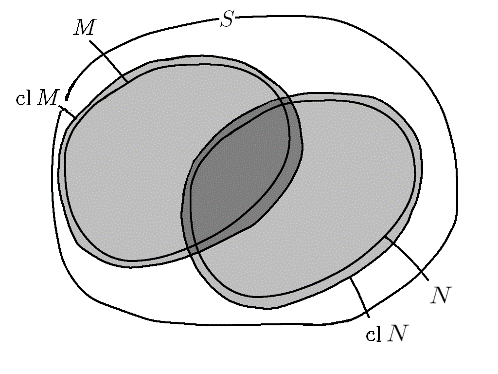
\includegraphics[width=80mm]{8.1.1.e.png}
\end{center}
\begin{proof}
位相空間$\left( S,\mathfrak{O} \right)$において、これの閉集合系$\mathfrak{A}$が与えられたとき、定理\ref{8.1.1.6}より$\emptyset \subseteq \emptyset$かつ$\mathfrak{\emptyset \in A}$かつ$\emptyset \subseteq A \land A \in \mathfrak{A} \Rightarrow \emptyset \subseteq A$が成り立つので、${\mathrm{cl}}\emptyset = \emptyset$が得られる。\par
$\forall M \in \mathfrak{P}(S)$に対し、定義より明らかに$M \subseteq {\mathrm{cl}}M$が成り立つ。\par
これにより、$\forall M,N \in \mathfrak{P}(S)$に対し、$M \cup N \subseteq {\mathrm{cl}}M \cup {\mathrm{cl}}N$が成り立つ。ここで、${\mathrm{cl}}M,{\mathrm{cl}}N\in \mathfrak{A}$より${\mathrm{cl}}M \cup {\mathrm{cl}}N\in \mathfrak{A}$かつ$M \cup N \subseteq A$なる任意の閉集合$A$を考えると、$M \subseteq A$かつ$A \in \mathfrak{A}$が成り立つなら、${\mathrm{cl}}M \subseteq A$が成り立つことと$N \subseteq A$かつ$A \in \mathfrak{A}$が成り立つなら、${\mathrm{cl}}N \subseteq A$が成り立つことより${\mathrm{int}}M \cup {\mathrm{int}}N \subseteq A$が得られる。したがって、定理\ref{8.1.1.6}より${\mathrm{cl}}(M \cup N) = {\mathrm{cl}}M \cup {\mathrm{cl}}N$が成り立つ。\par
$\forall M\in \mathfrak{P}(S)$に対し、${\mathrm{cl}}M \subseteq {\mathrm{cl}}M$かつ${\mathrm{cl}}M\in \mathfrak{A}$が成り立つかつ、${\mathrm{cl}}M \subseteq A$かつ$A \in \mathfrak{A}$が成り立つなら、${\mathrm{cl}}M \subseteq A$が成り立つことより${\mathrm{cl}}{{\mathrm{cl}}M} = {\mathrm{cl}}M$が得られる。
\end{proof}
\begin{thm}\label{8.1.1.14}
空集合$\emptyset$でない集合$S$の各部分集合たちにその集合$S$の部分集合たちを対応させる写像$a:\mathfrak{P}(S)\mathfrak{\rightarrow P}(S)$で次のことが成り立つとする。
\begin{itemize}
\item
  $a(\emptyset) = \emptyset$が成り立つ。
\item
  $\forall M \in \mathfrak{P}(S)$に対し、$M \subseteq a(M)$が成り立つ。
\item
  $\forall M,N \in \mathfrak{P}(S)$に対し、$a(M \cup N) = a(M) \cup a(N)$が成り立つ。
\item
  $a \circ a = a$が成り立つ。
\end{itemize}
このとき、その写像$aがその位相空間\left( S,\mathfrak{O} \right)$における閉包作用子と一致できる1つの位相$\mathfrak{O}$がただ1つに決まり、次式のように与えられる。
\begin{align*}
\mathfrak{O}=\left\{ S \setminus M \in \mathfrak{P}(S) \middle| a(M) = M \right\}
\end{align*}
\end{thm}\par
これを位相$\mathfrak{O}$の公理系とする場合があり、このときの公理系をKuratowskiの公理系という。
\begin{proof}
空集合$\emptyset$でない集合$S$の各部分集合たちにその集合$S$の部分集合たちを対応させる写像$a:\mathfrak{P}(S)\mathfrak{\rightarrow P}(S)$で次のことが成り立つとする。
\begin{itemize}
\item
  $a(\emptyset) = \emptyset$が成り立つ。
\item
  $\forall M \in \mathfrak{P}(S)$に対し、$M \subseteq a(M)$が成り立つ。
\item
  $\forall M,N \in \mathfrak{P}(S)$に対し、$a(M \cup N) = a(M) \cup a(N)$が成り立つ。
\item
  $a \circ a = a$が成り立つ。
\end{itemize}\par
ここで、$\mathfrak{O}=\left\{ S \setminus M \in \mathfrak{P}(S) \middle| a(M) = M \right\}$なる集合$\mathfrak{O}$が位相空間$\left( S,\mathfrak{O} \right)$における位相に、$\mathfrak{A} =\left\{ M \in \mathfrak{P}(S) \middle| a(M) = M \right\}$、即ち、$\mathfrak{A }=\left\{ M \in \mathfrak{P}(S) \middle| S \setminus M \in \mathfrak{O} \right\}$なる集合$\mathfrak{A}$がその位相空間$\left( S,\mathfrak{O} \right)$における閉集合系に一致しその写像$a$がその位相空間$\left( S,\mathfrak{O} \right)$の閉包作用子と一致することを示そう。\par
仮定とその集合$S$はその位相空間$\left( S,\mathfrak{O} \right)$でのどの集合にも含まれることより次のようになる。
\begin{align*}
a(\emptyset) = \emptyset \land S \subseteq a(S) \land a(S) \subseteq S &\Leftrightarrow a(S) = S \land a(\emptyset) = \emptyset\\
&\Leftrightarrow S,\emptyset \in \mathfrak{A}\\
&\Leftrightarrow S \setminus S,S \setminus \emptyset \in \mathfrak{O}\\
&\Leftrightarrow S,\emptyset \in \mathfrak{O}
\end{align*}
$\forall O,P \in \mathfrak{O}$に対し、仮定とこれの数学的帰納法より次のようになる。
\begin{align*}
O,P \in \mathfrak{O} &\Leftrightarrow a(S \setminus O) = S \setminus O \land a(S \setminus P) = S \setminus P\\
&\Rightarrow a(S \setminus O \cup S \setminus P) = a(S \setminus O) \cup a\left( S\setminus P \right) = S \setminus O \cup S \setminus P\\
&\Leftrightarrow S \setminus O \cup S \setminus P = S \setminus (O \cap P)\in \mathfrak{A}\\
&\Leftrightarrow O \cap P \in \mathfrak{O}
\end{align*}\par
任意の添数集合$\varLambda$によって添数づけられたその集合$\mathfrak{O}$の元の族$\left\{ O_{\lambda} \right\}_{\lambda \in \varLambda}$が与えられると、$\forall\lambda \in \varLambda$に対し、仮定より次のようになる。
\begin{align*}
O_{\lambda}\in \mathfrak{O} &\Leftrightarrow O_{\lambda}\in \mathfrak{O \land}O_{\lambda} \subseteq \bigcup_{\lambda \in \varLambda} O_{\lambda} \land S \setminus \bigcup_{\lambda \in \varLambda} O_{\lambda} \subseteq a\left( S \setminus \bigcup_{\lambda \in \varLambda} O_{\lambda} \right)\\
&\Leftrightarrow a\left( S \setminus O_{\lambda} \right) = S \setminus O_{\lambda} \land S \setminus \bigcup_{\lambda \in \varLambda} O_{\lambda} \subseteq S \setminus O_{\lambda} \land S \setminus \bigcup_{\lambda \in \varLambda} O_{\lambda} \subseteq a\left( S \setminus \bigcup_{\lambda \in \varLambda} O_{\lambda} \right)\\
&\Leftrightarrow a\left( S \setminus O_{\lambda} \right) = S \setminus O_{\lambda} \land S \setminus \bigcup_{\lambda \in \varLambda} O_{\lambda} \subseteq S \setminus O_{\lambda} \land S \setminus \bigcup_{\lambda \in \varLambda} O_{\lambda} \subseteq a\left( S \setminus \bigcup_{\lambda \in \varLambda} O_{\lambda} \right)\\
&\Rightarrow a\left( S \setminus O_{\lambda} \right) = S \setminus O_{\lambda} \land a\left( S \setminus \bigcup_{\lambda \in \varLambda} O_{\lambda} \right) \subseteq {\mathrm{cl}}\left( S \setminus O_{\lambda} \right) \land S \setminus \bigcup_{\lambda \in \varLambda} O_{\lambda} \subseteq a\left( S \setminus \bigcup_{\lambda \in \varLambda} O_{\lambda} \right)\\
&\Rightarrow a\left( S \setminus \bigcup_{\lambda \in \varLambda} O_{\lambda} \right) \subseteq S \setminus O_{\lambda} \land S \setminus \bigcup_{\lambda \in \varLambda} O_{\lambda} \subseteq a\left( S \setminus \bigcup_{\lambda \in \varLambda} O_{\lambda} \right)\\
&\Rightarrow a\left( S \setminus \bigcup_{\lambda \in \varLambda} O_{\lambda} \right) \subseteq \bigcap_{\lambda \in \varLambda} \left( S \setminus O_{\lambda} \right) \land S \setminus \bigcup_{\lambda \in \varLambda} O_{\lambda} \subseteq a\left( S \setminus \bigcup_{\lambda \in \varLambda} O_{\lambda} \right)\\
&\Leftrightarrow a\left( S \setminus \bigcup_{\lambda \in \varLambda} O_{\lambda} \right) \subseteq S \setminus \bigcup_{\lambda \in \varLambda} O_{\lambda} \land S \setminus \bigcup_{\lambda \in \varLambda} O_{\lambda} \subseteq a\left( S \setminus \bigcup_{\lambda \in \varLambda} O_{\lambda} \right)\\
&\Leftrightarrow a\left( S \setminus \bigcup_{\lambda \in \varLambda} O_{\lambda} \right) = S \setminus \bigcup_{\lambda \in \varLambda} O_{\lambda}\\
&\Leftrightarrow \bigcup_{\lambda \in \varLambda} O_{\lambda}\in \mathfrak{O}
\end{align*}\par
以上より次の条件たちが満たされその集合$\mathfrak{O}$は位相に相当する。
\begin{itemize}
\item
  $S,\emptyset \in \mathfrak{O}$が成り立つ。
\item
  $\forall O,P \in \mathfrak{O}$に対し、$O \cap P \in \mathfrak{O}$が成り立つ。
\item
  任意の添数集合$\varLambda$によって添数づけられたその集合$\mathfrak{O}$の元の族$\left\{ O_{\lambda} \right\}_{\lambda \in \varLambda}$において$\bigcup_{\lambda \in \varLambda} O_{\lambda}\in \mathfrak{O}$が成り立つ。
\end{itemize}\par
また、$\forall M \in \mathfrak{P}(S)$に対し、次のようになることから、
\begin{itemize}
\item
  $M \subseteq a(M)$が成り立つ。
\item
  $a \circ a(M) = a\left( a(M) \right) = a(M)$より$a(M)\in \mathfrak{A}$が成り立つ。
\item
  $M \subseteq A$かつ$A \in \mathfrak{A}$が成り立つなら、$a(M) \subseteq a(A) = A$が成り立つことにより、$a(M) \subseteq A$が成り立つ。
\end{itemize}
\ref{8.1.1.6}よりその集合$a(M)$はその集合$M$の閉包である。
\end{proof}
%\hypertarget{ux5916ux90e8ux3068ux5883ux754c}{%
\subsubsection{外部と境界}%\label{ux5916ux90e8ux3068ux5883ux754c}}
\begin{dfn}
位相空間$\left( S,\mathfrak{O} \right)$において、$M \in \mathfrak{P}(S)$なる集合$M$の補集合$S \setminus M$の開核${\mathrm{int}}(S \setminus M)$をその集合$M$の外部といい、${\mathrm{ext}}M$、$M^{e}$などと書く、即ち、次式のようになる。この外部$M^{e}$の元を外点という。
\begin{align*}
{\mathrm{ext}}M = {\mathrm{int}}(S \setminus M)
\end{align*}
\end{dfn}
これは次の図のように考えると、分かりやすかろう。
\begin{center}
  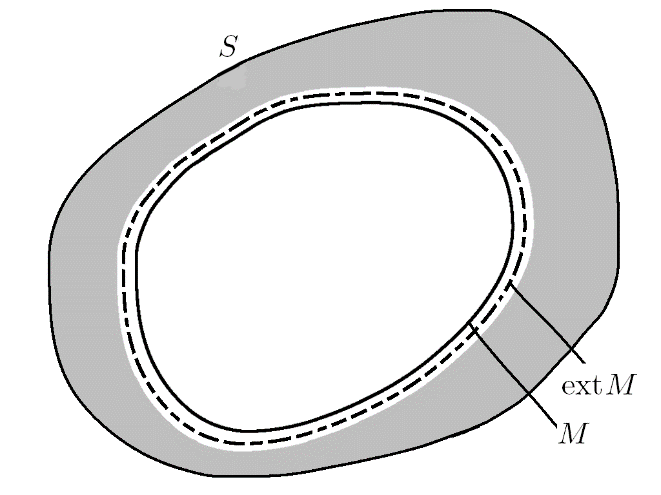
\includegraphics[width=76mm]{8.1.1.f.png}
\end{center}
\begin{thm}\label{8.1.1.15}
位相空間$\left( S,\mathfrak{O} \right)$において、$\forall M \in \mathfrak{P}(S)$に対し、次式が成り立つ\footnote{別の表記を用いれば、次のようになる。
\begin{align*}
  M^{e}&\in \mathfrak{O}\\
  M^{e} &= M^{ac}\\
  S &= M^{a} \sqcup M^{e}
  \end{align*}}。
\begin{align*}
{\mathrm{ext}}M&\in \mathfrak{O}\\
{\mathrm{ext}}M &= S \setminus {\mathrm{cl}}M\\
S &= {\mathrm{cl}}M \sqcup {\mathrm{ext}}M
\end{align*}
\end{thm}
\begin{proof}
これらは定義と開核と閉包との関係より明らかである。実際、位相空間$\left( S,\mathfrak{O} \right)$が与えられ$M \in \mathfrak{P}(S)$なる集合$M$において、開核は定義より位相$\mathfrak{O}$に属するので、${\mathrm{ext}}M = {\mathrm{int}}(S \setminus M)\in \mathfrak{O}$が成り立ち、開核と閉包との関係より${\mathrm{int}}(S \setminus M) = S \setminus {\mathrm{cl}}M$が成り立つので、${\mathrm{ext}}M = S \setminus {\mathrm{cl}}M$が成り立ち、これと差集合の性質より$S = {\mathrm{cl}}M \sqcup S \setminus {\mathrm{cl}}M = {\mathrm{cl}}M \sqcup {\mathrm{ext}}M$が成り立つ。
\end{proof}
\begin{dfn}
位相空間$\left( S,\mathfrak{O} \right)$において、$M \in \mathfrak{P}(S)$なる集合$M$の閉包${\mathrm{cl}}M$から開核${\mathrm{int}}M$への差集合${\mathrm{cl}}M \setminus {\mathrm{int}}M$をその集合$M$の境界といい、$\partial M$、$\partial(M)$、${bd}M$、$M^{f}$などと書く、即ち、次式のようになる。この境界$\partial M$の元を境界点という。
\begin{align*}
\partial M = {\mathrm{cl}}M \setminus {\mathrm{int}}M
\end{align*}
\end{dfn}\par
これは次の図のように考えると、分かりやすかろう。
\begin{center}
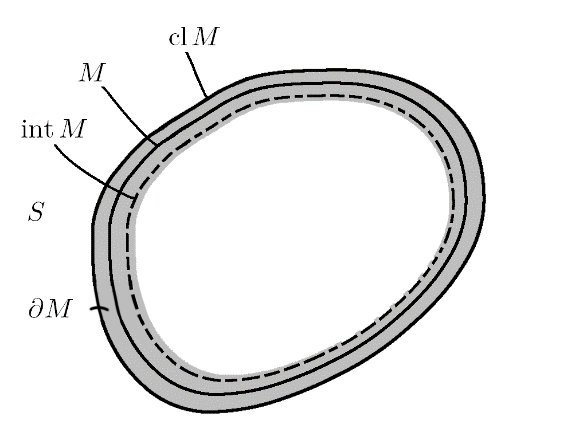
\includegraphics[width=76mm]{8.1.1.g.png}
\end{center}
\begin{thm}\label{8.1.1.16}
位相空間$\left( S,\mathfrak{O} \right)$において、$\forall M \in \mathfrak{P}(S)$に対し、次式が成り立つ\footnote{別の表記を用いれば、次のようになる。
\begin{align*}
  M^{a} &= M^{i} \sqcup M^{f}\\
  S &= M^{i} \sqcup M^{f} \sqcup M^{e}
\end{align*}}。
\begin{align*}
{\mathrm{cl}}M &= {\mathrm{int}}M \sqcup \partial M\\
S &= {\mathrm{int}}M \sqcup \partial M \sqcup {\mathrm{ext}}M
\end{align*}
\end{thm}
\begin{proof}
これらは定義より明らかである。実際、位相空間$\left( S,\mathfrak{O} \right)$が与えられ$M \in \mathfrak{P}(S)$なる集合$M$において、差集合の性質より${\mathrm{cl}}M = {\mathrm{int}}M \sqcup {\mathrm{cl}}M \setminus {\mathrm{int}}M = {\mathrm{int}}M \sqcup \partial M$が成り立ち、これと$S = {\mathrm{cl}}M \sqcup {\mathrm{ext}}M$が成り立つことにより、$S = {\mathrm{int}}M \sqcup \partial M \sqcup {\mathrm{ext}}M$が得られる。
\end{proof}
\begin{thm}\label{8.1.1.17}
位相空間$\left( S,\mathfrak{O} \right)$において、$\forall M \in \mathfrak{P}(S)$に対し、その集合$M$の境界$\partial(M)$は閉集合である。
\end{thm}
\begin{proof}
位相空間$\left( S,\mathfrak{O} \right)$とこれの閉集合系$\mathfrak{A}$、$M \in \mathfrak{P}(S)$なる集合$M$が与えられたとき、境界の定義より次のようになる。
\begin{align*}
S \setminus \partial M &= S \setminus \left( {\mathrm{cl}}M \setminus {\mathrm{int}}M \right)\\
&= S \setminus \left( {\mathrm{cl}}M \cap \left( S \setminus {\mathrm{int}}M \right) \right)\\
&= S \setminus {\mathrm{cl}}M \cup S \setminus S \setminus {\mathrm{int}}M\\
&= S \setminus {\mathrm{cl}}M \cup {\mathrm{int}}M
\end{align*}
ここで、${\mathrm{cl}}M\in \mathfrak{A}$が成り立つのであったので、閉集合の定義より$S \setminus {\mathrm{cl}}M\in \mathfrak{O}$が成り立つかつ、${\mathrm{int}}M\in \mathfrak{O}$が成り立つので、位相の定義より$S \setminus {\mathrm{cl}}M \cap {\mathrm{int}}M\in \mathfrak{O}$が成り立つ。したがって、$S \setminus \partial M \in \mathfrak{O}$が成り立ち閉集合の定義より$S \setminus \partial M$が成り立つ。
\end{proof}
\begin{thm}\label{8.1.1.18}
位相空間$\left( S,\mathfrak{O} \right)$において、$\forall M \in \mathfrak{P}(S)$に対し、その集合$M$が開集合であるならそのときに限り、積集合$M \cap \partial M$は空集合である、即ち、$M \in \mathfrak{O}$が成り立つならそのときに限り、$M \cap \partial M = \emptyset$が成り立つ。\par
これにより、開集合とはその集合自身の境界と交わらないような集合であることが分かる。
\end{thm}
\begin{proof}
位相空間$\left( S,\mathfrak{O} \right)$と$M \in \mathfrak{O}$なる集合$M$を考える。このとき、その集合$M$が開集合で$M = {\mathrm{int}}M$が成り立つので、したがって、$M \cap \partial M = \emptyset$が成り立つとすれば、
\begin{align*}
M \cap \partial M = \emptyset &\Leftrightarrow M \cap \left( {\mathrm{cl}}M \setminus {\mathrm{int}}M \right) = \emptyset\\
&\Leftrightarrow M \cap {\mathrm{cl}}M \cap S \setminus {\mathrm{int}}M = \emptyset\\
&\Leftrightarrow {\mathrm{cl}}M \cap M \cap S \setminus {\mathrm{int}}M = \emptyset\\
&\Leftrightarrow {\mathrm{cl}}M \cap M \cap S \setminus M = \emptyset\\
&\Leftrightarrow {\mathrm{cl}}M \cap \emptyset = \emptyset
\end{align*}
これは恒真式であるから、これより$M \in \mathfrak{O}$かつ$M \cap \partial M = \emptyset$は常に真であり、$M \in \mathfrak{O}$かつ$M \cap \partial M = \emptyset$が成り立つまたは$M \in \mathfrak{O}$、$M \cap \partial M = \emptyset$どちらも成り立たないということも真となりこれが同値にあたるので、$M \in \mathfrak{O}$が成り立つならそのときに限り、$M \cap \partial M = \emptyset$が成り立つことも真である。
\end{proof}
\begin{thm}\label{8.1.1.19}
位相空間$\left( S,\mathfrak{O} \right)$において、$\forall M \in \mathfrak{P}(S)$に対し、その集合$M$が閉集合であるならそのときに限り、その集合$M$はその境界$\partial M$を含む、即ち、その位相空間$\left( S,\mathfrak{O} \right)$の閉集合系を$\mathfrak{A}$として$M \in \mathfrak{A}$が成り立つならそのときに限り、$\partial M \subseteq M$が成り立つ。
\end{thm}
\begin{proof}
位相空間$\left( S,\mathfrak{O} \right)$とこれの閉集合系$\mathfrak{A}$、$M \in \mathfrak{A}$なる集合$M$を考える。このとき、閉集合の定義より$S \setminus M \in \mathfrak{O}$が成り立つので、${\mathrm{int}}(S \setminus M) = S \setminus M$が成り立ち$S \setminus {\mathrm{int}}(S \setminus M) = {\mathrm{cl}}M$より${\mathrm{cl}}M = M$が成り立つ。したがって、$\partial M \subseteq M$が成り立つとすれば、次式が成り立つ。
\begin{align*}
\partial M \subseteq M &\Leftrightarrow {\mathrm{cl}}M \setminus {\mathrm{int}}M \subseteq M\\
&\Leftrightarrow M \setminus {\mathrm{int}}M \subseteq M
\end{align*}
これは恒真式であるから、これより$M \in \mathfrak{A}$かつ$\partial M \subseteq M$は常に真であり、$M \in \mathfrak{A}$かつ$\partial M \subseteq M$が成り立つまたは$M \in \mathfrak{A}$、$\partial M \subseteq M$どちらも成り立たないということも真となりこれが同値にあたるので、$M \in \mathfrak{A}$が成り立つならそのときに限り、$\partial M \subseteq M$が成り立つことも真である。
\end{proof}
\begin{thm}\label{8.1.1.20}
位相空間$\left( S,\mathfrak{O} \right)$において、$\forall M \in \mathfrak{P}(S)$に対し、その集合$M$の境界点はその集合$M$の触点であるかつ、集合$S \setminus M$の触点でもある。
\end{thm}
\begin{proof}
位相空間$\left( S,\mathfrak{O} \right)$と$M \in \mathfrak{P}(S)$なる集合$M$が考えられれば、その集合$M$の位相的境界の定義より次のようになる。
\begin{align*}
a \in \partial M &= {\mathrm{cl}}M \setminus {\mathrm{int}}M\\
&= {\mathrm{cl}}M \cap \left( S \setminus {\mathrm{int}}M \right)\\
&= {\mathrm{cl}}M \cap {\mathrm{cl}}(S \setminus M)
\end{align*}
これが成り立つならそのときに限り、その元$a$はその集合$M$の触点であるかつ、集合$S \setminus M$の触点でもある。
\end{proof}
\begin{dfn}
位相空間$\left( S,\mathfrak{O} \right)$において、$\forall M \in \mathfrak{P}(S)$に対し、$a \in S$なる元$a$が集合$M \setminus \left\{ a \right\}$の触点であるとき、即ち、$a \in {\mathrm{cl}}\left( M \setminus \left\{ a \right\} \right)$が成り立つとき、その元$a$はその集合$M$の集積点という。
\end{dfn}
\begin{thm}\label{8.1.1.21}
位相空間$\left( S,\mathfrak{O} \right)$において、$\forall M \in \mathfrak{P}(S)$に対し、その集合$M$の集積点$a$はその集合$M$の触点の1つでもある。特に、$a \notin M$なるその集合$M$の全ての触点たち$a$はその集合$M$の集積点でもある。
\end{thm}
\begin{proof}
位相空間$\left( S,\mathfrak{O} \right)$が与えられ$M \in \mathfrak{P}(S)$なる任意の集合$M$とその集合$M$の集積点$a$において、$M \setminus \left\{ a \right\} \subseteq M$が成り立つので、${\mathrm{cl}}\left( M \setminus \left\{ a \right\} \right) \subseteq {\mathrm{cl}}M$が成り立つことにより、$a \in {\mathrm{cl}}M$が得られ、したがって、その集積点$a$はその集合$M$の触点の1つでもある。特に、$a \notin M$なるその集合$M$の任意の触点$a$について、$a \in {\mathrm{cl}}M$が成り立つかつ、$M \setminus \left\{ a \right\} = M$が成り立つので、$a \in {\mathrm{cl}}\left( M \setminus \left\{ a \right\} \right)$が成り立つ。
\end{proof}
\begin{dfn}
位相空間$\left( S,\mathfrak{O} \right)$において、$\forall M \in \mathfrak{P}(S)$に対し、$a \in M$なる元$a$でその集合$M$の集積点でないとき、その元$a$はその集合$M$の孤立点という。
\end{dfn}
%\hypertarget{ux8fd1ux508d}{%
\subsubsection{近傍}%\label{ux8fd1ux508d}}
\begin{dfn}
位相空間$\left( S,\mathfrak{O} \right)$において、$a \in S$なる元$a$が$V \in \mathfrak{P}(S)$なる集合$V$の内点である、即ち、$a \in {\mathrm{int}}V$が成り立つとき、その集合$V$がその元$a$の近傍であるという。
\end{dfn}\par
これは次の図のように考えると、分かりやすかろう。
\begin{center}
  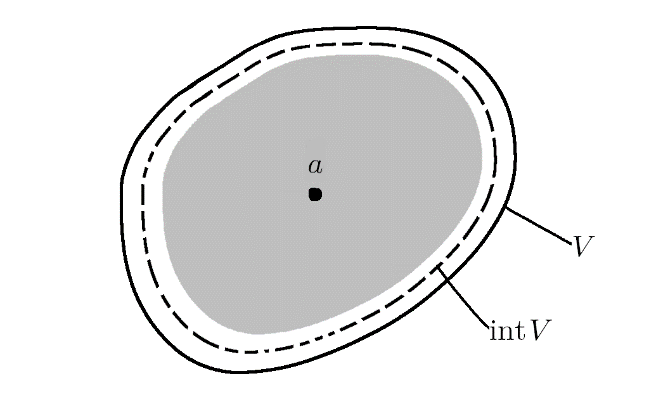
\includegraphics[width=74mm]{8.1.1.h.png}
\end{center}
\begin{dfn}
位相空間$\left( S,\mathfrak{O} \right)$において、$a \in S$なる元$a$の近傍全体の集合をその位相$\mathfrak{O}$におけるその元$a$の全近傍系といい、$\mathbf{V}(a)$などと書く、即ち、次式のように定義する。
\begin{align*}
\mathbf{V}(a) = \left\{ V \in \mathfrak{P}(S) \middle| a \in {\mathrm{int}}V \right\}
\end{align*}
\end{dfn}
\begin{thm}\label{8.1.1.22}
位相空間$\left( S,\mathfrak{O} \right)$において、$\forall a \in S$に対し、$V \in \mathbf{V}(a)$が成り立つならそのときに限り、$\exists O \in \mathfrak{O}$に対し、$a \in O \subseteq V$が成り立つ。
\end{thm}\par
これは次の図のように考えると、分かりやすかろう。
\begin{center}
  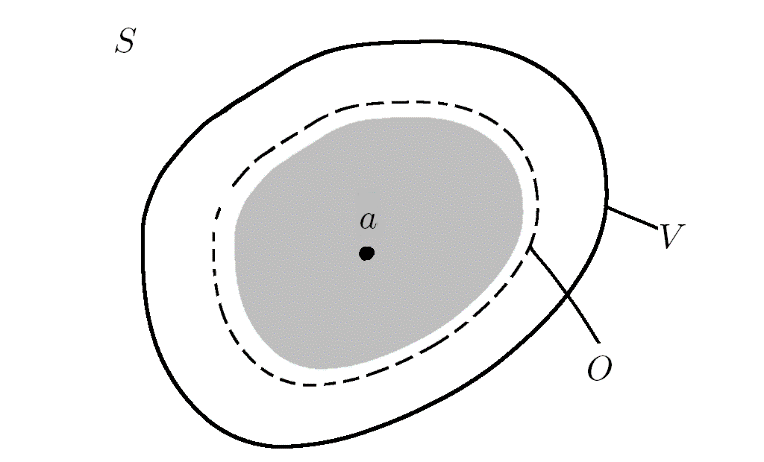
\includegraphics[width=88mm]{8.1.1.i.PNG}
\end{center}
\begin{proof}
位相空間$\left( S,\mathfrak{O} \right)$において、$\forall a \in S$に対し、$V \in \mathbf{V}(a)$が成り立つなら、開核と近傍の定義より$a \in {\mathrm{int}}V \subseteq V$が成り立つ。逆に、$a \in {\mathrm{int}}V$が成り立たないとき、$\exists O \in \mathfrak{O}$に対し、$a \in O \subseteq V$が成り立つ仮定すると、$a \in O = {\mathrm{int}}O \subseteq {\mathrm{int}}V$が得られるが、これは矛盾している。ゆえに、$a \in {\mathrm{int}}V$が成り立たないなら、$\forall O \in \mathfrak{O}$に対し、$a \notin O$が成り立つ、または、$O \subseteq V$が成り立たない。したがって、対偶律より$\exists O \in \mathfrak{O}$に対し、$a \in O \subseteq V$が成り立つなら、$V \in \mathbf{V}(a)$が成り立つ。
\end{proof}
\begin{thm}\label{8.1.1.23}
位相空間$\left( S,\mathfrak{O} \right)$において、$O \in \mathfrak{O}$が成り立つならそのときに限り、$\forall a \in O$に対し、$O \in \mathbf{V}(a)$が成り立つ。
これは次の図のように考えると、分かりやすかろう。
\begin{center}
  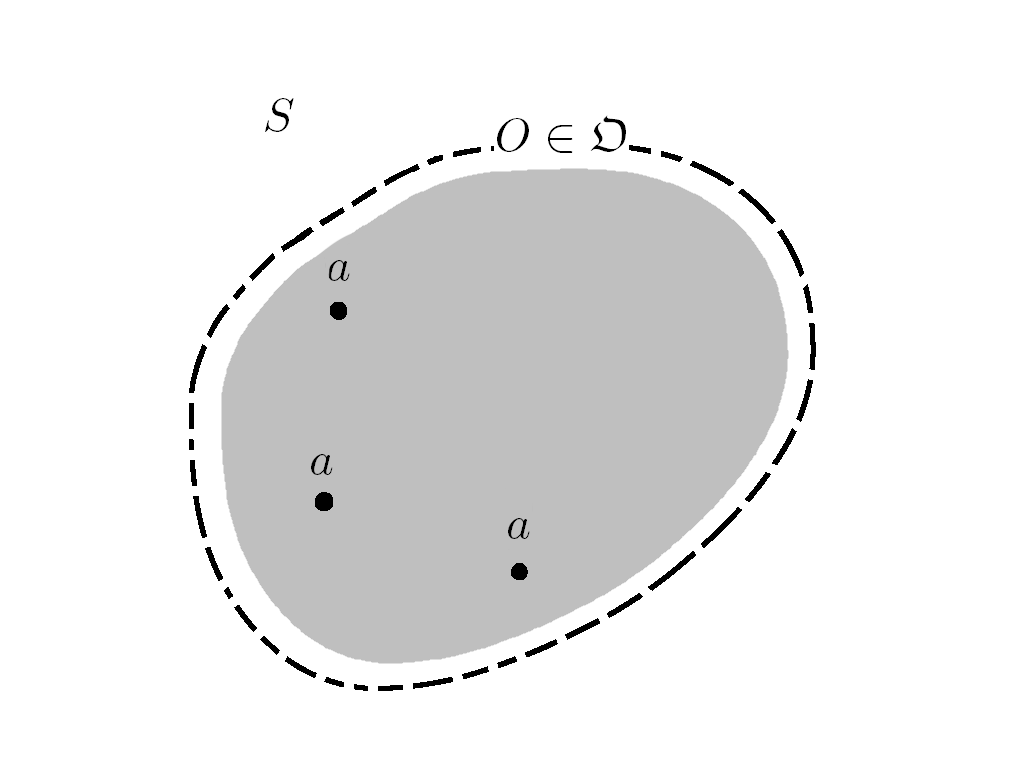
\includegraphics[width=92mm]{8.1.1.j.PNG}
\end{center}
\end{thm}
\begin{proof}
位相空間$\left( S,\mathfrak{O} \right)$において、$O \in \mathfrak{O}$が成り立つなら、$O = {\mathrm{int}}O$が成り立つので、$\forall a \in O$に対し、$a \in O = {\mathrm{int}}O$が成り立つ、即ち、$O \in \mathbf{V}(a)$が成り立つ。逆に、$\forall a \in O$に対し、$O \in \mathbf{V}(a)$が成り立つ、即ち、$a \in {\mathrm{int}}O$が成り立つなら、$O \subseteq {\mathrm{int}}O$が得られることになり、${\mathrm{int}}O \subseteq O$が成り立つので、$O = {\mathrm{int}}O$が成り立つ。これが成り立つならそのときに限り、その集合$O$は開集合である、即ち、$O \in \mathfrak{O}$が成り立つ。
\end{proof}
\begin{thm}\label{8.1.1.24}
位相空間$\left( S,\mathfrak{O} \right)$が与えられたとき、$\forall a \in S$に対し、その元$a$の全近傍系$\mathbf{V}(a)$について、次のことが成り立つ。
\begin{itemize}
\item
  $\forall V \in \mathbf{V}(a)$に対し、$a \in V$が成り立つ。
\item
  $\forall V \in \mathbf{V}(a)\forall W \in \mathfrak{P}(S)$に対し、$V \subseteq W$が成り立つなら、$W \in \mathbf{V}(a)$が成り立つ。
\item
  $\forall V,W \in \mathbf{V}(a)$に対し、$V \cap W \in \mathbf{V}(a)$が成り立つ。
\item
  $\forall V \in \mathbf{V}(a)\exists W \in \mathbf{V}(a)\forall b \in W$に対し、$V \in \mathbf{V}(b)$が成り立つ\footnote{例えば、$W = {\mathrm{int}}(V)$が挙げられる。}。
\end{itemize}
\end{thm}
これらの主張は次の図のように考えると、分かりやすかろう。
\begin{center}
  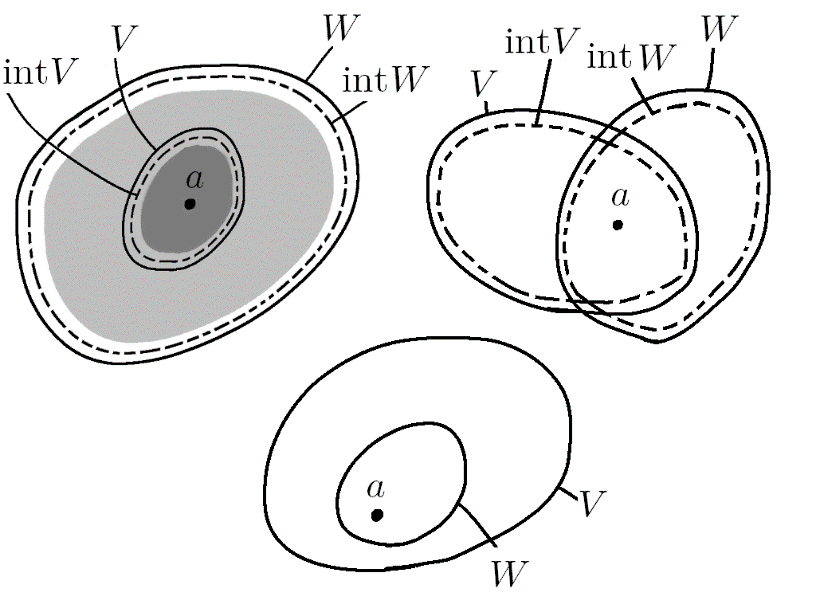
\includegraphics[width=94mm]{8.1.1.k.png}
\end{center}
\begin{proof}
位相空間$\left( S,\mathfrak{O} \right)$と$a \in S$なる元$a$の全近傍系$\mathbf{V}(a)$において、$\forall V \in \mathbf{V}(a)$に対し、定義より$a \in {\mathrm{int}}V$が成り立ち、${\mathrm{int}}V \subseteq V$が成り立つので、$a \in {\mathrm{int}}V \subseteq V$が得られる。よって、$a \in V$が成り立つ。\par
また、$\forall V \in \mathbf{V}(a)\forall W \in \mathfrak{P}(S)$に対し$V \subseteq W$が成り立つなら、定義より$a \in {\mathrm{int}}V$が成り立ち、${\mathrm{int}}V \subseteq V$が成り立つかつ、仮定より$V \subseteq W$が成り立つことより${\mathrm{int}}V \subseteq {\mathrm{int}}W$が成り立つので、$a \in {\mathrm{int}}V \subseteq {\mathrm{int}}W$が得られる。よって、$W \in \mathbf{V}(a)$が成り立つ。\par
$\forall V,W \in \mathbf{V}(a)$に対し、定義より$a \in {\mathrm{int}}V$かつ$a \in {\mathrm{int}}W$が成り立ち、したがって、$a \in {\mathrm{int}}V \cap {\mathrm{int}}W = {\mathrm{int}}(V \cap W)$が成り立つ。よって、$V \cap W \in \mathbf{V}(a)$が成り立つ。\par
$\forall V \in \mathbf{V}(a)$に対し、$W = {\mathrm{int}}V$とおけば、$\forall b \in W$に対し、$b \in W = {\mathrm{int}}V$が成り立つので、定義より$V \in \mathbf{V}(b)$が得られるかつ、$\forall a \in {\mathrm{int}}V$に対し、$a \in {\mathrm{int}}V = {\mathrm{int}}{{\mathrm{int}}V}$が成り立つので、定義より$W = {\mathrm{int}}V \in \mathbf{V}(a)$が成り立つ。よって、$\forall V \in \mathbf{V}(a)\exists W \in \mathbf{V}(a)\forall b \in W$に対し、$V \in \mathbf{V}(b)$が成り立つ。
\end{proof}
\begin{thm}\label{8.1.1.25}
空集合$\emptyset$でない集合$S$を用いて$a \in S$なる元々$a$に対するそれぞれ1つづつの空集合$\emptyset$でない集合$\mathfrak{P}(S)$の部分集合たち$\mathbf{V}(a)$が次のことが成り立つとする。
\begin{itemize}
\item
  $\forall V \in \mathbf{V}(a)$に対し、$a \in V$が成り立つ。
\item
  $\forall V \in \mathbf{V}(a)\forall W \in \mathfrak{P}(S)$に対し、$V \subseteq W$が成り立つなら、$W \in \mathbf{V}(a)$が成り立つ。
\item
  $\forall V,W \in \mathbf{V}(a)$に対し、$V \cap W \in \mathbf{V}(a)$が成り立つ。
\item
  $\forall V \in \mathbf{V}(a)\exists W \in \mathbf{V}(a)\forall b \in W$に対し、$V \in \mathbf{V}(b)$が成り立つ。
\end{itemize}
このとき、その集合$\mathbf{V}(a)$が位相空間$\left( S,\mathfrak{O} \right)$における$a \in S$なる元々$a$の全近傍系と一致できる1つの位相$\mathfrak{O}$がただ1つに決まり、次式のように与えられる。
\begin{align*}
\mathfrak{O}=\left\{ M \in \mathfrak{P}(S) \middle| a \in M \Rightarrow M \in \mathbf{V}(a) \right\}
\end{align*}
\end{thm}\par
これを位相の公理とするときがありこのような公理を全近傍系の公理という\footnote{もしかしたらぼくが一番好きな位相空間の公理かもしれません…。}。
\begin{proof}
空集合$\emptyset$でない集合$S$を用いて$a \in S$なる元々$a$に対するそれぞれ1つづつの空集合$\emptyset$でない集合$\mathfrak{P}(S)$の部分集合たち$\mathbf{V}(a)$が次のことが成り立つとする。
\begin{itemize}
\item
  $\forall V \in \mathbf{V}(a)$に対し、$a \in V$が成り立つ。
\item
  $\forall V \in \mathbf{V}(a)\forall W \in \mathfrak{P}(S)$に対し、$V \subseteq W$が成り立つなら、$W \in \mathbf{V}(a)$が成り立つ。
\item
  $\forall V,W \in \mathbf{V}(a)$に対し、$V \cap W \in \mathbf{V}(a)$が成り立つ。
\item
  $\forall V \in \mathbf{V}(a)\exists W \in \mathbf{V}(a)\forall b \in W$に対し、$V \in \mathbf{V}(b)$が成り立つ。
\end{itemize}
ここで、$\mathfrak{O}=\left\{ M \in \mathfrak{P}(S) \middle| a \in M \Rightarrow M \in \mathbf{V}(a) \right\}$なる集合$\mathfrak{O}$が位相空間$\left( S,\mathfrak{O} \right)$における位相に、その集合$\mathbf{V}(a)$が$a \in S$なる元$a$の全近傍系に一致することを示そう。\par
$\forall a \in S$に対し、仮定より$\exists V \in \mathbf{V}(a)$が成り立ち、その集合$\mathbf{V}(a)$がその集合$\mathfrak{P}(S)$の部分集合であるから、$V \subseteq S$が成り立つ。これにより、$S \in \mathbf{V}(a)$が成り立つ。また、明らかに$\mathfrak{\emptyset \in O}$が成り立つ。\par
$\forall O,P \in \mathfrak{O}$に対し、$O \cap P = \emptyset$が成り立つなら、上記より$O \cap P \in \mathfrak{O}$が成り立つ。$O \cap P \neq \emptyset$が成り立つなら、$\forall a \in S$に対し、$a \in O \cap P$が成り立つとき、その集合$\mathfrak{O}$の定義より$a \in O$が成り立つなら、$O \in \mathbf{V}(a)$が成り立つかつ、$a \in P$が成り立つなら、$P \in \mathbf{V}(a)$が成り立つので、$O,P \in \mathbf{V}(a)$が成り立つなら、$O \cap P \in \mathbf{V}(a)$が成り立ち、よって、$O \cap P \in \mathfrak{O}$が成り立つ。\par
任意の添数集合$\varLambda$によって添数づけられたその集合$\mathfrak{O}$の元の族$\left\{ O_{\lambda} \right\}_{\lambda \in \varLambda}$において、$\bigcup_{\lambda \in \varLambda} O_{\lambda} = \emptyset$が成り立つなら、上記より$\bigcup_{\lambda \in \varLambda} O_{\lambda}\in \mathfrak{O}$が成り立つ。$\bigcup_{\lambda \in \varLambda} O_{\lambda} \neq \emptyset$が成り立つなら、$\forall a \in S$に対し、$a \in \bigcup_{\lambda \in \varLambda} O_{\lambda}$が成り立つとき、$a \in O_{\lambda'}$なるその添数集合$\varLambda$の元$\lambda'$が存在して、$O_{\lambda'} \in \mathbf{V}(a)$が成り立つ。$O_{\lambda'} \subseteq \bigcup_{\lambda \in \varLambda} O_{\lambda}$が成り立つので、$\bigcup_{\lambda \in \varLambda} O_{\lambda} \in \mathbf{V}(a)$が成り立つ。よって、$\bigcup_{\lambda \in \varLambda} O_{\lambda}\in \mathfrak{O}$が成り立つ。\par
以上より次の条件たちが満たされその集合$\mathfrak{O}$は位相に相当する。
\begin{itemize}
\item
  $S,\emptyset \in \mathfrak{O}$が成り立つ。
\item
  $\forall O,P \in \mathfrak{O}$に対し、$O \cap P \in \mathfrak{O}$が成り立つ。
\item
  任意の添数集合$\varLambda$によって添数づけられたその集合$\mathfrak{O}$の元の族$\left\{ O_{\lambda} \right\}_{\lambda \in \varLambda}$において$\bigcup_{\lambda \in \varLambda} O_{\lambda}\in \mathfrak{O}$が成り立つ。
\end{itemize}\par
また、$S' = {\mathrm{int}}M$が成り立つことを次のこといづれも成り立つことと定め
\begin{itemize}
\item
  $S' \subseteq M$が成り立つ。
\item
  $S'\in \mathfrak{O}$が成り立つ。
\item
  $O \subseteq M$かつ$O \in \mathfrak{O}$が成り立つなら、$O \subseteq S'$が成り立つ。
\end{itemize}
$a \in {\mathrm{int}}V \Leftrightarrow V \in \mathbf{V}(a)$が成り立つことを示そう。\par
このとき、${\mathrm{int}}V\in \mathfrak{O}$が成り立つので、$a \in {\mathrm{int}}V \Rightarrow {\mathrm{int}}V \in \mathbf{V}(a)$が成り立ち、${\mathrm{int}}V \subseteq V$が成り立つので、以上より、$a \in {\mathrm{int}}V \Rightarrow V \in \mathbf{V}(a)$が成り立つ。\par
逆に、$\forall a \in S\forall V \in \mathbf{V}(a)$に対し、$U = \left\{ b \in S \middle| V \in \mathbf{V}(b) \right\}$なる集合$U$を考えよう。$b \in U$が成り立つなら、$V \in \mathbf{V}(b)$が得られ、したがって、$b \in V$が成り立つので、$U \subseteq V$が得られる。$\forall b \in U$に対し、$V \in \mathbf{V}(b)$が成り立ち、$\exists W \in \mathbf{V}(b)\forall c \in W$に対し、$V \in \mathbf{V}(c)$が成り立つのであったので、定義より$c \in U$が成り立ち$W \subseteq U$が得られ、$W \in \mathbf{V}(b)$より$W \subseteq U$が成り立つなら、$U \in \mathbf{V}(b)$が成り立つので、$b \in U \Rightarrow U \in \mathbf{V}(b)$が得られ、したがって、$U \in \mathfrak{O}$が成り立つ。$O \subseteq V$かつ$O \in \mathfrak{O}$が成り立つなら、$\forall d \in O$に対し、$O \in \mathbf{V}(d)$が成り立ち、したがって、$V \in \mathbf{V}(d)$が成り立つので、$d \in U$が成り立つ。したがって、$d \in O \Rightarrow d \in U$が得られ$O \subseteq U$が成り立つ。以上より、$U \subseteq V$かつ$U \in \mathfrak{O}$が成り立つかつ、$O \subseteq V$かつ$O \in \mathfrak{O}$が成り立つなら、$O \subseteq U$が成り立つので、$U = {\mathrm{int}}V$が成り立ち$V \in \mathbf{V}(a)$が成り立つなら、$a \in \left\{ b \in S \middle| V \in \mathbf{V}(b) \right\} = {\mathrm{int}}V$が得られ、したがって、$V \in \mathbf{V}(a) \Rightarrow a \in {\mathrm{int}}V$が成り立つ。\par
以上より、$a \in {\mathrm{int}}V \Leftrightarrow V \in \mathbf{V}(a)$が成り立つことが示された。
\end{proof}
\begin{thm}\label{8.1.1.26}
位相空間$\left( S,\mathfrak{O} \right)$において$\forall a \in S$に対し、その元$a$の1つの全近傍系$\mathbf{V}(a)$が与えられたとき、$\forall M \in \mathfrak{P}(S)$に対し、次のことが成り立つ。
\begin{itemize}
\item
  $a \in {\mathrm{int}}M$が成り立つならそのときに限り、$\exists V \in \mathbf{V}(a)$に対し、$V \subseteq M$が成り立つ。
\item
  $a \in {\mathrm{ext}}M$が成り立つならそのときに限り、$\exists V \in \mathbf{V}(a)$に対し、$V \cap M = \emptyset$が成り立つ。
\item
  $a \in {\mathrm{cl}}M$が成り立つならそのときに限り、$\forall V \in \mathbf{V}(a)$に対し、$V \cap M \neq \emptyset$が成り立つ。
\item
  $a \in \partial M$が成り立つならそのときに限り、$\forall V \in \mathbf{V}(a)$に対し、$V \cap M \neq \emptyset$かつ$V \cap S \setminus M \neq \emptyset$が成り立つ。
\end{itemize}
\end{thm}
\begin{proof}
位相空間$\left( S,\mathfrak{O} \right)$において$\forall a \in S$に対し、その元$a$の1つの全近傍系$\mathbf{V}(a)$が与えられたとき、$\forall M \in \mathfrak{P}(S)$に対し、$a \in {\mathrm{int}}M$が成り立つなら、$M \in \mathbf{V}(a)$より明らかに$\exists V \in \mathbf{V}(a)$に対し、$V \subseteq M$が成り立つ。逆に、$\exists V \in \mathbf{V}(a)$に対し、$V \subseteq M$が成り立つなら、$a \in {\mathrm{int}}V$が成り立つかつ${\mathrm{int}}V \subseteq {\mathrm{int}}M$が成り立つので、$a \in {\mathrm{int}}M$が得られる。\par
$a \in {\mathrm{ext}}M = {\mathrm{int}}(S \setminus M)$が成り立つならそのときに限り、上記の議論により$\exists V \in \mathbf{V}(a)$に対し、$V \subseteq S \setminus M$が成り立つ。このとき、次のようになることから、
\begin{align*}
V \subseteq S \setminus M &\Leftrightarrow \forall a \in S[ a \in V \Rightarrow a \in S \setminus M]\\
&\Leftrightarrow \forall a \in S\left[ a \notin V \vee (a \in S \land a \notin M) \right]\\
&\Leftrightarrow \forall a \in S\left[ (a \notin V \vee a \in S) \land (a \notin V \vee a \notin M) \right]\\
&\Leftrightarrow \forall a \in S[ a \notin V \vee a \in S] \land \forall a \in S\left[ \neg(a \in V \land a \in M) \right]\\
&\Leftrightarrow \forall a \in S[ a \in V \Rightarrow a \in S] \land \neg\exists a \in S[ a \in V \cap M]\\
&\Leftrightarrow V \subseteq S \land V \cap M = \emptyset\\
&\Leftrightarrow V \cap M = \emptyset
\end{align*}
これが成り立つならそのときに限り、$\exists V \in \mathbf{V}(a)$に対し、$V \cap M = \emptyset$が成り立つ。\par
$a \in {\mathrm{cl}}M$が成り立つならそのときに限り、$a \in S \setminus {\mathrm{int}}(S \setminus M)$が成り立つ、即ち、$a \notin {\mathrm{int}}(S \setminus M)$が成り立つ。そこで、上記の議論によりこれが成り立つならそのときに限り、$\forall V \in \mathbf{V}(a)$に対し、$V \cap M \neq \emptyset$が成り立つ。\par
$a \in \partial M$が成り立つならそのときに限り、$a \in {\mathrm{cl}}M$が成り立つかつ、$a \notin {\mathrm{int}}M$が成り立つ。これが成り立つならそのときに限り、上記の議論により、$\forall V \in \mathbf{V}(a)$に対し、$V \cap M \neq \emptyset$が成り立つかつ、$\forall V \in \mathbf{V}(a)$に対し、$V \subseteq M$が成り立たない。このとき、次のようになることから、
\begin{align*}
\neg V \subseteq M &\Leftrightarrow \neg\forall a \in S[ a \in V \Rightarrow a \in M]\\
&\Leftrightarrow \exists a \in S\left[ \neg(a \notin V \vee a \in M) \right]\\
&\Leftrightarrow \exists a \in S[ a \in V \land a \notin M]\\
&\Leftrightarrow \exists a \in S[ a \in V \land a \in S \setminus M]\\
&\Leftrightarrow \exists a \in S[ a \in V \cap S \setminus M]\\
&\Leftrightarrow V \cap S \setminus M \neq \emptyset
\end{align*}
これが成り立つならそのときに限り、$\forall V \in \mathbf{V}(a)$に対し、$V \cap M \neq \emptyset$が成り立つかつ、$\forall V \in \mathbf{V}(a)$に対し、$V \cap S \setminus M \neq \emptyset$が成り立つ、即ち、$\forall V \in \mathbf{V}(a)$に対し、$V \cap M \neq \emptyset$かつ$V \cap S \setminus M \neq \emptyset$が成り立つ。
\end{proof}
\begin{thebibliography}{50}
\bibitem{1}
  松坂和夫, 集合・位相入門, 岩波書店, 1968. 新装版第2刷 p152-165 ISBN978-4-00-029871-1
\bibitem{2}
  川平友規. "第3章 位相空間の基礎のキソ". 一橋大学. \url{http://www.math.titech.ac.jp/~kawahira/courses/kiso/03-isou.pdf} (2021-1-10 取得)
\bibitem{3}
  きいねく. "大学数学の難関分野:【位相空間論】とは一体何なのか?". note. \url{https://note.com/keyneqq/n/na8d370a26bff} (2022-3-26 18:04 閲覧)
\bibitem{4}
  桂田祐史. "数学解析 第11回~開集合と閉集合(1)~". 明治大学. \url{http://nalab.mind.meiji.ac.jp/~mk/lecture/kaiseki-2021/K11_0628_handout.pdf} (2022-3-26 18:12 取得)
\end{thebibliography}
\end{document}
